\documentclass[11pt,a4paper]{article}
\usepackage[margin=28mm]{geometry}
\usepackage{amsthm}
\newtheorem{theorem}{Theorem}
\newtheorem{proposition}{Proposition}
\newtheorem{lemma}{Lemma}
\newtheorem{corollary}{Corollary}
\usepackage[T1]{fontenc}
\usepackage[utf8]{inputenc}
\usepackage{lmodern}
\usepackage{amsmath,amssymb,mathtools}
\usepackage{microtype,booktabs,tabularx,array}
\usepackage{graphicx}
\usepackage{tikz}
\usepackage[hidelinks]{hyperref}
\usepackage{bookmark}
\DeclareMathOperator{\conv}{conv}
\DeclareMathOperator{\dist}{dist}
\DeclareMathOperator{\Lip}{Lip}
\DeclareMathOperator{\rank}{rank}
\DeclareMathOperator{\row}{row}
\DeclareMathOperator{\vol}{vol}
\newcommand{\R}{\mathbb R}
\newcommand{\one}{\mathbf 1}
\newcommand{\Hu}{\mathsf H}
\newcommand{\norm}[1]{\lVert#1\rVert_\infty}
\newcommand{\eps}{\varepsilon}
\newcommand{\Laff}{L_{\mathrm{aff}}}
\newcommand{\Llip}{L_{\mathrm{Lip}}}
\newcommand{\loss}{\mathcal L}
\newcommand{\link}[2]{\href{#1}{#2}}
\setlength{\emergencystretch}{1em}


\usepackage{xurl}
\newcommand{\doi}[1]{\href{https://doi.org/#1}{doi:\nolinkurl{#1}}}
\hypersetup{bookmarksnumbered=true,pdfsubject={Tropical abstract domains and neural network certification}}

\hypersetup{pdftitle={Contextual Precision in Tropical Abstract Domains: Sharp Generator Budgets and ReLU Certificates},pdfauthor={Nassim Arifette}}
\title{Contextual Precision in Tropical Abstract Domains:\\Sharp Generator Budgets and ReLU Certificates}
\input{authors}
\date{September 2026}
\begin{document}
\maketitle
\begin{abstract}
Exact representation of a state does not ensure precision after a tropical join. We calculate worst contextual observation loss for normalized max-plus hulls under a linear consistency slice. For an arbitrary compact invariant and continuous observation, compact witness fibers give an attained formula using finitely many context points. For the signed diagonal, every finite enclosure contains a canonical partition representative with no larger generator budget. This makes the resulting minimax laws exhaustive over arbitrary ambient generators. The optimal Lipschitz loss is $1/[2(M-1)]$; affine losses have a different dimension dependence and an exact all-budget formula for dimensions at least four. We apply the theory to continuous rational ReLU classifiers. Under a specified hidden-state merge before a nonlinear suffix, every exact three-generator diagonal summary loses the classification certificate, while four generators recover the exact positive margin. An affine-readout contract converts generator budgets into sufficient margin guarantees. We also realize worst contextual losses by continuous ReLU paths with finite axial context representations, keeping the dependence on the chosen representative explicit. Written proofs and exact rational checks support these claims; no performance advantage on trained networks is asserted.
\end{abstract}
\noindent\textbf{Keywords:} abstract interpretation; tropical convexity; contextual precision; neural network certification.
\section{Introduction}
When an analyzer combines paths, the choice of representation can matter even if each incoming state has an exact concretization. Signed tropical domains make the distinction explicit: an ambient representative stores both a variable and its negative, while concretization enforces their consistency. Inconsistent ambient points can become consistent after a join. Exactness at the current program point therefore does not guarantee precision for a later query.

\paragraph{A neural analysis decision.}
Consider input subdivision for a ReLU classifier. An analyzer may retain geometric summaries of hidden regions and merge them before analyzing the suffix. Section~\ref{sec:nonlinear-application} fixes a connected-input rational network whose nonlinear ReLU suffix has true minimum margin $1/8$. Every exact three-generator diagonal summary gives a merged minimum $-1/8$. Replacing the coarse anchor by two refined anchors recovers the exact $1/8$ margin with four generators. Neither the network nor the property changes. An affine-readout example follows in Section~\ref{sec:relu-application}. Precise per-region queries avoid the loss, so the policy choice is part of both results.

Tropical neural analysis~\cite{goubault2021} provides the motivating signed representation and subdivision setting. We ask a complementary quantitative question: what loss can a finite representative incur after a specified operation, and which representative minimizes that loss? This is a question about abstract-domain design, not another approximation of the ReLU transformer. It is related to quantitative incompleteness~\cite{campion2023} but seeks exact resource laws for one concrete domain and observation model.

\paragraph{Contributions.}
First, Theorem~\ref{thm:observation} calculates worst finite-context loss for every fixed continuous observation under a linear lift and compact invariant. Second, Theorem~\ref{thm:partition} shows that arbitrary diagonal enclosures contain a canonical partition summary with no larger generator budget. Without this step, optimizing partition anchors would not establish optimality over all representatives. Third, exact cell costs give the Lipschitz law $1/[2(M-1)]$, the affine dimension dependence, and every affine budget for $n\ge4$ (Theorems~\ref{thm:lipschitz}--\ref{thm:budget}). Finally, we realize affine obstructions as continuous ReLU networks, prove the fixed-classifier separation, and derive a sufficient budget for preserving certified margins.

The resource is the number of finite ambient generators. The concrete contexts, consistency slice, invariant and observation norm are fixed explicitly; a retained disjunction is not a tropical join. Our laws do not imply equal runtime costs or handle arbitrary abstract operands. The neural construction is an analytic application with exact arithmetic checks, not evidence of gains on trained networks. Section~\ref{sec:evidence} separates these claims from empirical ones and compares the classical ingredients with the problem-specific reductions. The fixed-normal ordinary-union rate in Appendix~\ref{app:dictionary} is a complementary theorem with a different budget.

\section{Normalized Hulls and Contextual Observations}\label{sec:contexts}
All state and generator coordinates are finite real numbers. We use the infinity norm for geometry. For $U\subseteq\R^p$, a normalized tropical combination is
\[
z=\max_{1\le k\le r}(u^k+\lambda_k\one_p),\qquad
u^k\in U,\quad \lambda_k\le0,\quad \max_k\lambda_k=0.
\]
Its finite-combination hull is $\Hu(U)$. Inactive coefficients may be $-\infty$ and may be omitted. The homogeneous coordinate is $z_0=u_0^k=0$; it records the normalization. For a nonempty compact $U$, this hull is compact: at most $p+1$ operands suffice, by retaining one attaining operand per coordinate including coordinate zero. If $U\subseteq[-R,R]^p$, coefficients below $-2R$ can be raised to $-2R$ without changing the maximum. The hull is therefore a continuous image of a compact parameter set. No additional closure is needed here.

Let $A:\R^n\to\R^p$ have rows $a_1,\ldots,a_p$, and set $a_0=0$. The concretization of $P$ is $A^{-1}P$. A finite representative is $P=\Hu\{g^1,\ldots,g^M\}$. Fix a nonempty compact invariant $K$ with nonempty $S=K\cap A^{-1}P$. For finite $T\subseteq K$, including $T=\varnothing$, define
\begin{equation}\label{eq:join-loss}
J_T^K(P)=K\cap A^{-1}\Hu(P\cup AT),\qquad
\ell_\varphi(P,T)=\min_{S\cup T}\varphi-\min_{J_T^K(P)}\varphi.
\end{equation}
The function $\varphi:K\to\R$ is continuous. Both minima exist and the loss is nonnegative, since $S\cup T\subseteq J_T^K(P)$. This baseline changes if the initial slice changes; comparisons of representatives below always keep it fixed.

\paragraph{Sector convention.}
For $i=0,\ldots,p$, let
\[
\Sigma_i=\{v\in\R^p:v_i\le v_j\ (0\le j\le p)\},\qquad v_0=0.
\]
The classical sector criterion~\cite[Prop.~1.1]{hill2020} reads
\begin{equation}\label{eq:sectors}
\Hu(U)=\bigcap_{i=0}^p(U+\Sigma_i).
\end{equation}
For completeness, $z\in u+\Sigma_i$ means that $u+(z_i-u_i)\one_p\le z$, with equality in coordinate $i$ and coefficient $z_i-u_i\le0$. One such operand per coordinate, including zero, yields a normalized combination. The converse follows by choosing an attaining operand. The sign convention matters in pulling this criterion back through $A$.

For the signed lift write $E(x)=(x,-x)$, $K_n=[0,1]^n$, and $D_n=\{t\one_n:0\le t\le1\}$. For this diagonal use the coarse representative
\begin{equation}\label{eq:p0}
P_0=\Hu\{E(0),E(\one_n),(0_n,-\one_n)\},
\end{equation}
whose exactness follows from the partition identity in Section~\ref{sec:partitions}.

\section{Recovering a Certificate Before a Nonlinear ReLU Suffix}\label{sec:nonlinear-application}
The first application fixes the whole network, input region and merge policy. Changing the diagonal representative alone recovers the \emph{exact} classification margin. The suffix is nonlinear at the hidden-state cut, so the affine zero-loss result in dimension two does not apply.

\paragraph{Network and specification.}
For $t\in[0,3]$, let $\sigma(s)=\max(0,s)$ and
\begin{align*}
F_1(t)&=\sigma(t-1)-\tfrac74\sigma(t-2),\\
F_2(t)&=\tfrac34-\tfrac34\sigma(t)+\tfrac74\sigma(t-1)-\sigma(t-2).
\end{align*}
The hidden image traverses $(0,3/4)\to(0,0)\to(1,1)\to(1/4,1)$. It is $R=V\cup D_2\cup H$, where $V=\{(0,s):0\le s\le3/4\}$ and $H=\{(s,1):1/4\le s\le1\}$. The prefix uses one width-three ReLU layer and a width-two affine/ReLU layer; the latter ReLU is the identity on $K_2$.

Put $z^\star=(1/4,3/4)$ and take logits $g_1(z)=\norm{z-z^\star}$, $g_2(z)=1/8$. An explicit standard ReLU suffix computes
\[
h=(\sigma(z_1-1/4),\sigma(1/4-z_1),\sigma(z_2-3/4),\sigma(3/4-z_2)),
\]
then $k_1=\sigma(h_1+h_2-h_3-h_4)$, $k_2=\sigma(h_3+h_4)$, and $g_1=k_1+k_2$. Thus the full architecture is $1\to3\to2\to4\to2\to2$, with an affine output. Since $\dist_\infty(z^\star,R)=1/4$, its true minimum margin $\psi=g_1-g_2$ is $1/8$.

\paragraph{Fixed merge interface.}
Split the input at $1$ and $2$ and represent all three hidden segments exactly. For the axial segments use
\begin{align*}
U_V&=\Hu\{E(0,0),E(0,3/4),(0,0,0,-3/4)\}=V\times(-V),\\
U_H&=\Hu\{E(1,1),E(1/4,1),(1/4,1,-1,-1)\}=H\times(-H).
\end{align*}
For the diagonal use either $P_3=\Hu\{E(0),E(\one_2),c(0,1)\}$ or
\[
P_4=\Hu\{E(0),E(\one_2),c(0,1/2),c(1/2,1)\},\qquad
c(a,b)=(a,a,-b,-b).
\]
The merged state is $A_i=K_2\cap E^{-1}\Hu(P_i\cup U_V\cup U_H)$. Evaluate the suffix exactly on this state; additional suffix-relaxation error is outside this comparison.

\begin{proposition}[Exact certificate recovery]\label{prop:nonlinear-recovery}
The true minimum margin is $1/8$, while $\min_{A_3}\psi=-1/8$ and $\min_{A_4}\psi=1/8$. Every exact diagonal representative with at most three finite generators fails for this fixed interface. Four diagonal generators suffice and are minimal. After shared endpoints are counted once, the displayed full merge lists contain seven and eight generators, respectively; no minimality of that total is claimed.
\end{proposition}
\begin{proof}
Let $g=c(0,1)$ and $p=(1/4,1/4,-3/4,-3/4)$. We have
\begin{align*}
p&=\max\{g,E(0)-\tfrac34\one_4,E(\one_2)-\tfrac34\one_4\}\in P_3,\\
E(z^\star)&=\max\{p,E(1/4,1)-\tfrac14\one_4,E(0,3/4)-\tfrac14\one_4\}.
\end{align*}
Both combinations are normalized, so $z^\star\in A_3$. Since $\psi\ge-1/8$ everywhere, this gives the exact abstract minimum. Theorem~\ref{thm:partition} places $P_3$ inside every admissible three-generator diagonal representative, preserving the witness.

A normalized combination yielding $E(x)\in\Hu(P_4\cup U_V\cup U_H)$ has a coefficient-zero generator dominated by $E(x)$. For the two refined diagonal anchors this forces $x\in[0,1/2]^2$ or $[1/2,1]^2$. For the axial anchors it forces $x\in V$ or $H$; a consistent endpoint forces equality to that endpoint. Thus
\[
A_4\subseteq V\cup H\cup[0,1/2]^2\cup[1/2,1]^2.
\]
Every point in this cover is at distance at least $1/4$ from $z^\star$: on the lower square use coordinate two, on the upper square coordinate one, and on $V,H$ their fixed coordinates. Hence $\psi\ge1/8$. The reachable diagonal point $(1/2,1/2)$ attains this bound. Budgets below three cannot represent the diagonal, completing minimality.
\end{proof}

\begin{figure}[t]
\centering
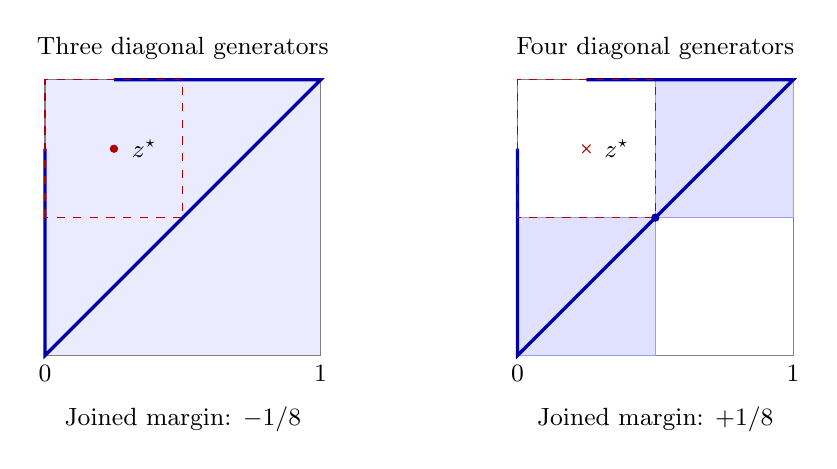
\begin{tikzpicture}[x=3.5cm,y=3.5cm,font=\small]
\begin{scope}
\fill[blue!8] (0,0) rectangle (1,1);
\draw[gray] (0,0) rectangle (1,1);
\draw[very thick,blue!65!black] (0,.75)--(0,0)--(1,1)--(.25,1);
\draw[red!70!black,dashed] (0,.5) rectangle (.5,1);
\fill[red!70!black] (.25,.75) circle (1.5pt);
\node[right] at (.28,.75) {$z^\star$};
\node[below] at (0,0) {$0$};\node[below] at (1,0) {$1$};
\node[above] at (.5,1.04) {Three diagonal generators};
\node[below] at (.5,-.15) {Joined margin: $-1/8$};
\end{scope}
\begin{scope}[xshift=6.0cm]
\fill[blue!12] (0,0) rectangle (.5,.5);
\fill[blue!12] (.5,.5) rectangle (1,1);
\draw[gray] (0,0) rectangle (1,1);
\draw[blue!40] (0,0) rectangle (.5,.5);
\draw[blue!40] (.5,.5) rectangle (1,1);
\draw[very thick,blue!65!black] (0,.75)--(0,0)--(1,1)--(.25,1);
\draw[red!70!black,dashed] (0,.5) rectangle (.5,1);
\draw[red!70!black] (.235,.735)--(.265,.765) (.235,.765)--(.265,.735);
\node[right] at (.28,.75) {$z^\star$};
\fill[blue!65!black] (.5,.5) circle (1.5pt);
\node[below] at (0,0) {$0$};\node[below] at (1,0) {$1$};
\node[above] at (.5,1.04) {Four diagonal generators};
\node[below] at (.5,-.15) {Joined margin: $+1/8$};
\end{scope}
\end{tikzpicture}

\caption{The blue path is the same exact reachable set in both panels. Shading shows the diagonal anchors' necessary cover for consistent joined states, not the exact joined set; the axial operands add $V$ and $H$. The dashed square has radius $1/4$ about $z^\star$. The refined cover avoids its interior, certifying the distance margin.}\label{fig:recovery}
\end{figure}

\paragraph{Meaning of the intervention.}
The refined anchors replace the coarse anchor; simply adjoining generators would retain its spurious state. The guarantee concerns exact suffix evaluation on the merged set, not the bounds of an unspecified heuristic solver. Querying the three regions separately or retaining their disjunction also certifies the network. Reusable hidden-state summaries are a possible reason to merge, but neither reuse nor partitioning is new~\cite{fischer2021,singh2019}. The example demonstrates a representation choice at that interface; its frequency and cost on trained models are empirical questions.

The axial representatives above behave like their concrete segments even in arbitrary ambient joins. Appendix~\ref{app:neural-transfer} proves this fact and uses safe axial connectors to realize worst affine and Lipschitz contextual losses by continuous ReLU networks. The realizing network may depend on the representative, and connector storage is an additional resource. Section~\ref{sec:relu-application} gives a distinct affine-readout contract; its positive lower bound is not claimed to recover the exact margin.

\section{Exact Contextual Loss and Fidelity}
\subsection{An exact formula for a fixed observation}
A coordinate $i$ is \emph{covered by $P$ at $x$} when some generator satisfies
\[
(a_j-a_i)\cdot x\ge g_j^k-g_i^k\qquad(0\le j\le p).
\]
Let $I_P(x)$ be the uncovered coordinates, with $g_0^k=0$. Its witness fibers are
\begin{equation}\label{eq:fibers}
F_i(x)=\{t\in K:(a_j-a_i)\cdot(t-x)\le0\ (0\le j\le p)\}.
\end{equation}
Each fiber is compact and contains $x$. By~\eqref{eq:sectors},
\begin{equation}\label{eq:missing}
x\in J_T^K(P)\quad\Longleftrightarrow\quad
T\cap F_i(x)\ne\varnothing\quad\hbox{for all }i\in I_P(x).
\end{equation}
The coverage test may use the displayed generators: a coordinate supplied by a combination from $P$ is supplied by an attaining generator in that combination.

\begin{theorem}[Worst loss of a fixed observation]\label{thm:observation}
For arbitrary linear $A$, nonempty compact $K$, finite $P$, and nonempty $S=K\cap A^{-1}P$, put $m_S=\min_S\varphi$. Then
\begin{equation}\label{eq:observation}
\sup_{T\subseteq K\text{ finite}}\ell_\varphi(P,T)
=\max_{x\in K}\left[\min\left\{m_S,
        \min_{i\in I_P(x)}\max_{t\in F_i(x)}\varphi(t)\right\}-\varphi(x)\right].
\end{equation}
Here $\min\varnothing=+\infty$. The maximum is nonnegative and is attained by a context with at most $p+1$ points.
\end{theorem}
\begin{proof}
Write $d_\varphi(x)$ for the bracketed expression. Given $T$, choose a minimizer $x$ on $J_T^K(P)$. Each missing coordinate has a witness $t_i\in T\cap F_i(x)$. Therefore
\[
\min_{S\cup T}\varphi\le
\min\{m_S,\min_{i\in I_P(x)}\max_{F_i(x)}\varphi\},
\]
which bounds the loss by $d_\varphi(x)$. Conversely, for a fixed $x$, choose a maximizer of $\varphi$ on each missing fiber. The resulting $T$ has at most $p+1$ points, places $x$ in the join, and has concrete minimum equal to the bracket's first term. Its loss is at least $d_\varphi(x)$.

It remains to justify the maximum despite changing coverage. The graph of $F_i$ is closed in $K\times K$, hence $b_i(x)=\max_{F_i(x)}\varphi$ is upper semicontinuous. The set where coordinate $i$ is covered is closed, being a finite union of closed inequality systems. Replace $b_i$ by $\max_K\varphi$ on that closed set. The replacement is still upper semicontinuous and does not affect the minimum with $m_S$. Taking the minimum over all coordinates and subtracting $\varphi$ proves upper semicontinuity of $d_\varphi$. At a minimizer on $S$, all coordinates are covered and $d_\varphi=0$. Compactness and the two inequalities above prove the statement.
\end{proof}

No convexity of $K$ or injectivity of $A$ enters this proof. Pointwise values $d_\varphi(x)$ may be negative; only their maximum is nonnegative.

\begin{corollary}[Affine and Lipschitz observations]\label{cor:observations}
For affine observations, additive constants cancel. Their worst loss with $\|w\|_1\le1$ is
\begin{equation}\label{eq:affine-support}
\loss_{\rm aff}(P)=\max_{\substack{x\in K\\\|w\|_1\le1}}
\min\left\{\min_{s\in S}w\cdot(s-x),
   \min_{i\in I_P(x)}\max_{t\in F_i(x)}w\cdot(t-x)\right\}.
\end{equation}
For all $1$-Lipschitz observations on $K$, the worst loss is
\begin{equation}\label{eq:radius}
\loss_{\rm Lip}(P)=\max_{x\in K}
\min\left\{\dist_\infty(x,S),\min_{i\in I_P(x)}r_i(x)\right\},
\quad r_i(x)=\max_{t\in F_i(x)}\norm{t-x}.
\end{equation}
Both maxima and finite witnessing contexts are attained.
\end{corollary}
\begin{proof}
Substitute $\varphi(t)=w\cdot t$ in Theorem~\ref{thm:observation}. The same upper semicontinuity argument on the compact product with the unit $1$-norm ball gives attainment. For a Lipschitz observation, each difference $\varphi(t)-\varphi(x)$ is bounded by $\norm{t-x}$, as is the difference to a nearest point of $S$. At a maximizing $x$, the radial function $\varphi(t)=\norm{t-x}$ attains every bound simultaneously. Fiber radii have the same compactness and upper semicontinuity properties.
\end{proof}

For the signed lift $E(x)=(x,-x)$ and a box $K=[l,u]$, the fibers have a simple form. $F_0(x)=\{x\}$; in $F_{+j}(x)$ the displacement $h=t-x$ has $h_j=\norm h\ge0$, and in $F_{-j}(x)$ it has $-h_j=\norm h\ge0$. Consequently
\begin{equation}\label{eq:signed-radii}
r_0(x)=0,\qquad r_{+j}(x)=u_j-x_j,\qquad r_{-j}(x)=x_j-l_j.
\end{equation}
A missing homogeneous coordinate prevents positive loss for either class.

\subsection{Exact states and unbounded contexts}\label{sec:unbounded}
The bounded-context formula also clarifies why current-state exactness is insufficient. We give a structural comparison for contexts in all of $\R^n$; its distant witnesses cannot be used unchanged in a fixed invariant.

Define the pulled-back cones and interior-row indices
\[
C_i^A=\{h:(a_j-a_i)\cdot h\ge0\ \forall j\},\qquad
I_A=\{i:a_i\in\operatorname{int}_{\R^n}\conv\{a_0,\ldots,a_p\}\}.
\]
Normal-cone duality gives $i\in I_A$ exactly when $C_i^A=\{0\}$. The interior is ambient, not relative. By sectors,
$A^{-1}\Hu(AS)=\bigcap_i(S+C_i^A)$ for compact nonempty $S$.
Thus $A^{-1}\Hu(AS)=S$ for every such $S$ exactly when $I_A\ne\varnothing$: sufficiency is immediate; otherwise choose nonzero $h_i\in C_i^A$ and $S=\{-h_i\}_i$, whose reconstruction contains zero although $S$ does not. When $I_A\ne\varnothing$, $A$ is injective and $\Hu(AS)$ is finitely generated exactly when $S$ is finite. Indeed, a generator supplying an interior coordinate of $As$ must equal $As$: expressing it as a combination of points of $AS$, an attaining operand has displacement in $C_i^A=\{0\}$. This concerns the \emph{ideal hull}, not larger finite representatives with the same slice.

For $P=\Hu(G)$ and $S=A^{-1}P\ne\varnothing$, put
\begin{align}
Q_i(g)&=\{x:(a_j-a_i)\cdot x\ge g_j-g_i\ \forall j\},\nonumber\\
C_A(P)&=\bigcap_{i\in I_A}\ \bigcup_{g\in G}Q_i(g).\label{eq:defect-set}
\end{align}
If $I_A\ne\varnothing$, this is a compact set containing $S$, since each nonempty $Q_i(g)$ has recession cone $\{0\}$ for $i\in I_A$.

\begin{proposition}[Unbounded concrete-context fidelity]\label{prop:fidelity}
Assume $I_A\ne\varnothing$. For every finite $T\subseteq\R^n$,
\[
S\cup T\subseteq A^{-1}\Hu(P\cup AT)\subseteq C_A(P)\cup T.
\]
Every $x\in C_A(P)\setminus S$ can be exposed by at most $p+1-|I_A|$ context points at any prescribed positive infinity-norm distance from $x$. Hence all concrete-context joins are exact iff $C_A(P)=S$, and the worst Lipschitz minimum loss is
\[
\max_{x\in C_A(P)}\dist_\infty(x,S).
\]
\end{proposition}
\begin{proof}
If a joined point $x$ is not in $T$, an interior coordinate cannot be supplied by a context: its fiber in $\R^n$ is $\{x\}$. All such coordinates must be covered by $P$, proving the upper inclusion. For a noninterior index $i$, choose $h_i$ with $\norm{h_i}=1$ and
$a_i\cdot h_i=\max_j a_j\cdot h_i\ge0$. Then $t_i=x+Rh_i$ supplies coordinate $i$ with coefficient $-R a_i\cdot h_i\le0$. The covered interior coordinates are supplied by $P$; coordinate zero is supplied by one of these sources, so normalization holds. This proves exposure. For the loss upper bound, any spurious point is in $C_A(P)$ and lies within the displayed distance of $S$. For equality, choose a maximizing $x$, use $R$ at least this distance, and observe with $\varphi(z)=\norm{z-x}$.
\end{proof}

For the signed lift, $I_E=\{0\}$ and $C_E(P)=\bigcup_{(u,v)\in G}[u,-v]$, omitting empty boxes. Finite representatives faithful for all concrete contexts therefore exist exactly for finite unions of axis-aligned boxes. For a box $[l,u]$, take the ambient box $[l,u]\times[-u,-l]$: it has a finite tropical generating set consisting of its lower corner and one point raising each coordinate separately to its upper bound. Its slice and its defect set both equal $[l,u]$. Joining these representatives handles a finite union. A nonconstant continuous graph on a connected box is not such a union: any box contained in a graph has constant output, and a finite continuous image of a connected set is a point. Nevertheless $P_0$ represents the diagonal exactly. Fidelity is the stronger requirement.

Concrete and abstract operands are also different. With $A(t)=(t,2t,3t)$, take
\[
P=\Hu\{(0,0,0),(1,1,2)\},\quad
Q=\Hu\{(1,2,3),(0,1,1)\}.
\]
Here $I_A=\{1,2\}$, $C_A(P)=A^{-1}P=\{0\}$ and $C_A(Q)=A^{-1}Q=\{1\}$. Both are faithful for every concrete context. But
\[
\max\{(1,1,2)-\tfrac12\one_3,(0,1,1)\}
=(\tfrac12,1,\tfrac32)=A(\tfrac12).
\]
Their abstract join is inexact. If there is just one interior index, the union in~\eqref{eq:defect-set} does commute with the join, giving a sufficient condition for faithful abstract joins. This is not a classification for several interior indices.

\section{Arbitrary Generators Reduce to Partitions}\label{sec:partitions}
From now on $E(x)=(x,-x)$, $K_n=[0,1]^n$, and $D_n=\{t\one_n:0\le t\le1\}$. Admissible representatives have the \emph{global} exact slice $E^{-1}P=D_n$ and at most $M$ finite generators. Write
\begin{equation}\label{eq:minimax}
L_{\mathcal O}(M,n)=\inf_{\substack{P=\Hu(G),\ |G|\le M\\ E^{-1}P=D_n}}
\ \sup_{\substack{T\subseteq K_n\text{ finite}\\\varphi\in\mathcal O}}
\left(\min_{D_n\cup T}\varphi-\min_{J_T^{K_n}(P)}\varphi\right).
\end{equation}
We use $\Llip$ for $1$-Lipschitz observations and $\Laff$ for affine observations with $\|w\|_1\le1$. Real generator coordinates are allowed; the budget does not charge bit complexity.

For a partition $0=t_0<\cdots<t_q=1$, define
\begin{equation}\label{eq:partition-rep}
\begin{split}
P_{\boldsymbol t}&=\Hu\{e^0,e^1,c(t_{i-1},t_i):1\le i\le q\},\\
e^0&=E(0),\quad e^1=E(\one_n),\quad c(a,b)=(a\one_n,-b\one_n).
\end{split}
\end{equation}
Every point of this hull has constant positive and negative blocks, so its slice is contained in $D_n$. Conversely, for $a\le t\le b$,
\[
E(t\one_n)=\max\{c(a,b),e^0-t\one_{2n},e^1-(1-t)\one_{2n}\},
\]
which proves exactness.

\begin{theorem}[Contained partition representative]\label{thm:partition}
If $E(D_n)\subseteq P=\Hu\{g^1,\ldots,g^M\}$, then $M\ge3$ and $P$ contains a partition representative with at most $M-2$ cells. For exact $P$, replacing it by that representative weakly improves every contextual observation loss. Consequently the infima in~\eqref{eq:minimax} equal the infima over partitions with at most $M-2$ cells.
\end{theorem}
\begin{proof}
For $g=(u,v)$, define its anchor interval
$I_g=[0,1]\cap[\max_j u_j,\min_j(-v_j)]$.
The intervals cover $[0,1]$: a normalized representation of $E(t\one_n)$ has a coefficient-zero generator dominated by that point. Two distinct generators have no positive-length anchor. A generator attaining coordinate $-1$ at $e^0$ satisfies $v_1\ge0$ and $u_1\le v_1$, so its anchor ends at most at zero. A generator attaining coordinate $+1$ at $e^1$ satisfies $u_1\ge1$ and $v_1\le u_1-2$, so its anchor starts at least at one. The two inequalities on $u_1-v_1$ are incompatible for the same generator. The positive-length anchors alone still cover $[0,1]$, since their finite closed union contains the complement of finitely many points. There are at most $M-2$ of them.

Greedily choose an anchor reaching farthest right from the current endpoint. This yields a subordinate partition using at most one cell per chosen anchor. If $[a,b]\subseteq I_g$, then
\begin{equation}\label{eq:anchor-containment}
c(a,b)=\max\{g,e^0-b\one_{2n},e^1-(1-a)\one_{2n}\}\in P.
\end{equation}
The endpoint vectors belong to $P$ even if they are not displayed generators. This normalized identity proves containment. For exact inputs, both slices equal $D_n$ and joining a contained representative yields a contained result with the same concrete reference minimum. This proves the minimax reduction.
\end{proof}

Containment holds even for an inexact initial enclosure; comparing losses with different initial slices does not follow. The reduction changes the ambient set. It is not redundancy deletion preserving that set, nor a restriction of competitors to symmetric generators.

\subsection{Local cell costs and the exact Lipschitz law}
The homogeneous coordinate is covered for $P_{\boldsymbol t}$ exactly on the union of the anchor cubes $[t_{i-1},t_i]^n$. Outside that union there is no positive deficit. Inside one cube, write $u=\min_j x_j$, $v=\max_j x_j$. If $u<v$, the missing positive coordinates are precisely those with $x_j>u$, and the missing negative coordinates those with $x_j<v$. All constant-block generators can supply only extremal coordinates; the two endpoints supply all covered extrema. This description agrees with $P_0$ on each cube, including shared boundaries. Hence either observation class has partition loss equal to the maximum of its cell costs.

By~\eqref{eq:radius} and~\eqref{eq:signed-radii}, the pointwise Lipschitz deficit is
$\min\{(v-u)/2,u,1-v\}$.
For $n\ge2$, its maximum over $[a,b]^n$ is
\begin{equation}\label{eq:lipcell}
V(a,b)=\min\{(b-a)/2,b/3,(1-a)/3,1/4\}.
\end{equation}
Indeed, a deficit at least $\eta$ is feasible iff
$\max(a,\eta)+2\eta\le\min(b,1-\eta)$, giving these four bounds. Two coordinate values suffice for attainment.

\begin{theorem}[Exact Lipschitz generator law]\label{thm:lipschitz}
For $n\ge2$ and $M\ge3$,
\[
\Llip(M,n)=\frac1{2(M-1)}.
\]
An optimal partition with $q=M-2\ge2$ cells has boundary widths $3\delta$ and interior widths $2\delta$, where $\delta=1/[2(q+1)]$. For $q=1$ its cost is $1/4$. For $n=1$ the loss is zero.
\end{theorem}
\begin{proof}
The stated widths give the upper bound by~\eqref{eq:lipcell}. For a partition with $q\le M-2$ cells and maximum cost $\ell<1/4$, each cell $[a,b]$ has $b-a\le2\ell$, or $b\le3\ell$, or $a\ge1-3\ell$. Group the cells satisfying the second condition, then the remaining cells satisfying the third, then all other cells. The first two groups each cover length at most $3\ell$ when nonempty; each remaining cell covers at most $2\ell$. Thus the total length is at most $2(q+1)\ell$. Since it is one, $\ell\ge1/[2(M-1)]$. If $\ell\ge1/4$ the conclusion is immediate. Theorem~\ref{thm:partition} makes the bound exhaustive. Finally $D_1=K_1$, so there are no spurious states after clipping in dimension one.
\end{proof}

\subsection{A classical partition certificate}\label{sec:partition-certificate}
Let $W(a,b)$ be any nonnegative cell cost monotone under interval inclusion. Given two weak $q$-cell partitions $\boldsymbol s,\boldsymbol t$, some cell of $\boldsymbol t$ contains the corresponding cell of $\boldsymbol s$: take the first $i\ge1$ with $t_i\ge s_i$. Thus
\begin{equation}\label{eq:partition-certificate}
\min_i W(s_{i-1},s_i)\le
\inf_{\boldsymbol t}\max_i W(t_{i-1},t_i)\le
\max_i W(s_{i-1},s_i).
\end{equation}
An equal-cost partition is therefore globally optimal. The lower certificate must have exactly $q$ cells; a partition with fewer cells suffices only for the upper bound. Weak partitions allow zero widths and encode smaller budgets by repeated knots.

This interval-containment and balancing principle is classical~\cite[Lemma~2.12]{tilli2019}. We use sufficiency of equal costs, not uniqueness or necessity that every optimizer equalize. Non-strictly monotone costs may have plateaus. The specific work below is to compute the contextual cell cost and construct a feasible equal-cost partition.

\section{Affine Observations: Coefficients and Cell Costs}\label{sec:affine}
Let $d_n(x,w)$ denote the pointwise expression in~\eqref{eq:affine-support} for $P_0$, $S=D_n$, $K=K_n$, and define
\begin{equation}\label{eq:affine-cell}
W_n(a,b)=\max_{\substack{x\in[a,b]^n\\\|w\|_1\le1}}d_n(x,w).
\end{equation}
The partition loss is $\max_i W_n(t_{i-1},t_i)$. In particular, all contexts still range over the \emph{global} cube; restricting them to the cell would define a different problem. We have $0\le W_n(a,b)\le(b-a)/2$ by the Lipschitz bound, and $W_n$ is monotone under interval inclusion.

\subsection{A bound that includes covered extrema}
Suppose $\delta=d_n(x,w)>0$. Homogeneity lets us normalize $\|w\|_1=1$. Both signs must occur, since otherwise the diagonal baseline is nonpositive. Write the positive coefficients as $a_i>0$, the negative magnitudes as $c_j>0$, and
\[
A=\sum_i a_i,\quad C=\sum_j c_j=1-A,\quad p=|\{i:w_i>0\}|,\quad k=|\{j:w_j<0\}|.
\]
Zeros remain in the geometry; $p+k\le n$.

\begin{lemma}[Uniform coefficient inequalities]\label{lem:coefficient}
Every nonzero coefficient has magnitude strictly less than $1/2$, and
\begin{equation}\label{eq:coefficients}
\delta\le(1-2a_i)x_i,\qquad
\delta\le(1-2c_j)(1-x_j).
\end{equation}
If $u=\sum_i a_ix_i/A$, $v=\sum_j c_jx_j/C$, $\alpha=1-2A/p$, $\beta=1-2C/k$, and $m=\min(A,C)$, then
\begin{equation}\label{eq:means}
\delta\le\alpha u,\qquad
\delta\le\beta(1-v),\qquad
\delta\le m-Au-C(1-v).
\end{equation}
In particular $u<v$.
\end{lemma}
\begin{proof}
If the negative $i$-sector is missing, a witness displacement satisfies $h_i=-r$, $|h_j|\le r$, $0\le r\le x_i$. Its affine increment is at most $(1-2a_i)r$. Thus positivity forces $a_i<1/2$ and yields the first inequality. If that sector is covered, $x_i=\max_jx_j$. The diagonal baseline gives
\[
\delta\le\min(0,A-C)-w\cdot x
\le-w\cdot x\le(C-a_i)x_i\le(1-2a_i)x_i.
\]
This handles the extremum without invoking a missing-sector constraint. Reflection $x\mapsto\one_n-x$, $w\mapsto-w$ proves the negative-coefficient inequality.

The function $f(t)=t/(1-2t)$ is convex on $(0,1/2)$, with $f''(t)=4/(1-2t)^3$. Multiplying $x_i\ge\delta/(1-2a_i)$ by $a_i$ and summing yields $Au\ge\delta A/\alpha$. The negative case is identical. The third inequality in~\eqref{eq:means} is the exact diagonal baseline. It is positive only if $u<v$.
\end{proof}

At most two coefficients cannot have total magnitude one with each magnitude less than $1/2$. Thus $\Laff(M,n)=0$ for $n\le2$, unlike the Lipschitz loss when $n=2$.

\begin{theorem}[Smallest-budget dimension law]\label{thm:dimension}
For $M=3$,
\[
\Laff(3,n)=
\begin{cases}
0,&n\le2,\\
(5\sqrt5-11)/2,&n=3,\\
\displaystyle\frac1{4+1/(p-1)+1/(k-1)},&
n\ge4,\quad p=\lfloor n/2\rfloor,\ k=\lceil n/2\rceil .
\end{cases}
\]
The representative $P_0$ attains these values.
\end{theorem}
\begin{proof}
Theorem~\ref{thm:partition} reduces three generators to the sole cell $[0,1]$. Summing~\eqref{eq:coefficients} with the diagonal baseline and applying Jensen gives
\begin{equation}\label{eq:jensen-global}
\delta\le\frac{\min(A,C)}{1+\sum_i f(a_i)+\sum_j f(c_j)}
\le\frac{\min(A,C)}{1+A/(1-2A/p)+C/(1-2C/k)}.
\end{equation}
If one sign group is a singleton of magnitude $c<1/2$, its term alone gives
\[
\delta\le\frac{c(1-2c)}{2(1-c)^2}\le\frac18;
\]
the difference from $1/8$ is $(1-3c)^2/[8(1-c)^2]$. In dimension three, $p=2,k=1$ up to reflection, and the full bound is $c^2(1-2c)/(1-c)^2$. With $r=c/(1-c)$ this becomes $r^2(1-r)/(1+r)$, whose derivative has the sign of $1-r-r^2$. Its maximum is the stated golden-ratio value. An attaining context is given in Appendix~\ref{app:three}.

For $p,k\ge2$ and $A\le1/2$, the reciprocal of the last expression in~\eqref{eq:jensen-global} is
\[
\frac1A+\frac p{p-2A}+\frac{k(1-A)}{A(k-2+2A)}.
\]
The first two terms have derivative at most $-4+2p/(p-1)^2\le0$, and the third is strictly decreasing. Reflection gives the optimum at $A=C=1/2$. Its value is $U(p,k)=1/[4+1/(p-1)+1/(k-1)]$, increasing in each count and largest at balanced counts totaling $n$.

To attain it, put $\alpha=1-1/p$, $\beta=1-1/k$, $\delta=U(p,k)$, $u=\delta/\alpha$, and $v=1-\delta/\beta$. Then $u<1/2<v$, $v-u=2\delta$, and choose
\[
x=(u^p,v^k),\qquad w=((1/(2p))^p,(-1/(2k))^k).
\]
Here exponents denote repeated coordinates. For each low coordinate, use a displacement $-u$ at that coordinate, $+u$ at other low coordinates, and $-u$ at high coordinates. For each high coordinate, use $r=1-v$ there and at low coordinates, and $-r$ at the other high coordinates. These contexts stay in the cube and have affine value zero; their support increments are $\alpha u=\beta r=\delta$. They supply all missing sectors. The endpoints and the coefficient-zero anchor supply the rest, so the loss is $\delta$. In particular two signs of each kind attain $1/6>1/8$, excluding singleton optima when $n\ge4$.
\end{proof}

\subsection{Interior and boundary cells}
\begin{lemma}[Interior cells]\label{lem:interior}
If $h=b-a\le\min(a,1-b)$, then
\[
W_3(a,b)=\frac{h\max(a,1-b)}{2-h},\qquad
W_n(a,b)=h/2\quad(n\ge4).
\]
\end{lemma}
\begin{proof}
For $n\ge4$ the upper bound is distance to the diagonal. For attainment take two low coordinates $a$, two high coordinates $b$, coefficients $(1,1,-1,-1)/4$, and zero coefficients elsewhere. Put other coordinates at $a$. In each missing sector, a displacement of radius $h$ stays in the cube. Force the required coordinate to the appropriate extremum and move other positive-weight coordinates up and negative-weight coordinates down. The affine increment is $h/2$ if the forced coordinate has nonzero weight, and $h$ otherwise. The baseline is $h/2$, so~\eqref{eq:affine-support} proves equality. The dimension-three calculation is provided in Appendix~\ref{app:three}; it uses~\eqref{eq:coefficients}, not an assumed symmetry of the maximizer.
\end{proof}

Boundary cells require singleton signs even when $n\ge4$. We give the reduction needed for their exact evaluation. It also explains the all-cell scalar formulas in Appendix~\ref{app:allcells}.

\begin{lemma}[Boundary reduction]\label{lem:boundary-reduction}
For $0<b\le1/2$, let $d=n-3\ge0$, $0<c<1/2$, $A=1-c$, $\alpha=1-2A/(n-1)$, and $\gamma=1-2c$. Then $W_n(0,b)$ is the maximum of
\begin{align}
&\frac{(n-3)b}{3n-8}\quad(n\ge4),\label{eq:balanced-boundary}\\
&\max_{0\le s\le b}\frac{s(b-s)}{2-s},\label{eq:positive-boundary}\\
&\max_{0<c<1/2}\min\left\{\frac{\alpha cb}{\alpha+A},
                  \frac{c}{1+A/\alpha+c/\gamma}\right\}.\label{eq:negative-boundary}
\end{align}
All positive branch values have two-level attainers with equal coefficients within each sign group.
\end{lemma}
\begin{proof}
The averages in~\eqref{eq:means} lie in $[0,b]$. If both sign groups have at least two coefficients, ignore the second inequality and increase $v$ to $b$. For $A\ge1/2$ the remaining bound is $\alpha Cb/(A+\alpha)$, decreasing with $A$. For $A\le1/2$, put $B=A-C(1-b)$. The bound is the positive part of $\alpha B/(A+\alpha)$, increasing with $A$ wherever positive: with $e=2/p$, its derivative numerator is $(2-b)(\alpha^2-eA^2)+(1-b)>0$, since $\alpha^2-eA^2\ge1-2A$. Hence $A=C=1/2$ is best. Increasing $p$ to $n-2$ gives~\eqref{eq:balanced-boundary}. It is attained with $u=b/(1+2\alpha)$, $v=b$, $p=n-2$, $k=2$: low missing supports are $\alpha u$, high missing supports are $1/4$, and the baseline is $(b-u)/2$.

If the positive group is a singleton, $A<1/2$ and $\alpha=1-2A$. The same relaxation is attained at $u=B/(1-A)$ when $B>0$, $v=b$, splitting the negative mass equally. Set $s=1-A/(1-A)$. A positive value requires $0<s<b$ and becomes $s(b-s)/(2-s)$. High-sector supports do not bind: their excess over the baseline is $C(1-1/k)-A(v-u)>0$, because $C>A$, $k\ge2$, and $v-u\le1/2$.

For a negative singleton, let $C=c<1/2$ and allocate any unused coordinates to the positive group, so $p=n-1$. For $\delta>0$, \eqref{eq:means} is feasible exactly when
\[
\delta+A\max(0,\delta/\alpha)+c\max(1-b,\delta/\gamma)\le c.
\]
Expanding the maxima leaves the two bounds in~\eqref{eq:negative-boundary}; the other two bounds $cb$ and $\gamma c/A$ are weaker. Conversely set $u=\delta/\alpha$ and $v=\min(b,1-\delta/\gamma)$. The baseline forces $0\le u<v\le b$. Equal positive coefficients at $u$ and the negative singleton at $v$ have missing supports $\alpha u$ and $\gamma(1-v)$, so they attain the bound. These cases exhaust all sign patterns. Positivity of every coefficient bound handles zeros and excludes groups of two singletons.
\end{proof}

\section{The Exact Affine Budget Law in Dimensions at Least Four}\label{sec:budgets}
For $d=n-3\ge0$ and $0<c<1/2$, define
\begin{align}
D_d(c)&=2(d+1)-dc,&
k_d(c)&=\frac{c(d+2c)}{D_d(c)},\nonumber\\
B_d(c)&=\frac{(1-2c)D_d(c)}{2(d+1)(1-c)^2},&
F_d(c)&=\frac{c(d+2c)(1-2c)}{2(d+1)(1-c)^2}.\label{eq:boundary-functions}
\end{align}
Thus $F_d=k_dB_d$. The endpoint extensions have $B_d(0)=1$, $B_d(1/2)=0$, and $F_d(0)=F_d(1/2)=0$.

\begin{theorem}[Exact boundary cost]\label{thm:boundary}
For $0<b\le1/2$, let $c_d(b)$ be the unique root of $B_d(c)=b$ in $(0,1/2)$ and put $N_d(b)=F_d(c_d(b))$. Then
\begin{equation}\label{eq:boundary-cost}
W_n(0,b)=
\begin{cases}
N_0(b)=\displaystyle b\left(\frac{\sqrt{1-b}}{1+\sqrt{1-b}}\right)^2,&n=3,\\[3pt]
\max\{\kappa_d b,N_d(b)\},\quad \kappa_d=d/(3d+1),&n\ge4.
\end{cases}
\end{equation}
At $b=0$ the cost is zero. Reflection gives $W_n(1-b,1)=W_n(0,b)$.
\end{theorem}
\begin{proof}
Substitution in~\eqref{eq:negative-boundary} gives $\max_c\min\{k_d(c)b,F_d(c)\}$. The derivatives are
\begin{align*}
k_d'(c)&=\frac{2d(d+1)+8(d+1)c-2dc^2}{D_d(c)^2}>0,\\
B_d'(c)&=-\frac{d+(d+4)c}{2(d+1)(1-c)^3}<0,\\
F_d'(c)&=\frac{d(1-3c)+4c(1-3c+c^2)}{2(d+1)(1-c)^3}.
\end{align*}
Let $r=(3-\sqrt5)/2$. The last numerator is negative for $c>r$, while
\[
B_d(r)=\frac{(1-2r)(2-r)}{2(1-r)^2}
       +\frac{r(1-2r)}{2(d+1)(1-r)^2}>\frac12,
\]
because the first term is $1/2$. Therefore $c_d(b)>r$ for $b\le1/2$. Below the crossing, $k_d(c)b\le k_d(c_d(b))b$; above it, $F_d(c)\le F_d(c_d(b))$. At the crossing the two coincide, proving the singleton maximum without a global unimodality assumption.

The positive-singleton branch is bounded by $b^2/[4(2-b)]\le b/12$. For $d\ge1$ the balanced branch is at least $b/4$ and dominates it. For $d=0$, $B_0(2/5)=5/9>1/2$ implies $N_0(b)>4b/25>b/12$. Thus the positive singleton never determines a boundary cost. Solving $B_0(c)=b$ gives the displayed dimension-three formula.
\end{proof}

The root needed here is quadratic:
\begin{equation}\label{eq:boundary-quadratic}
2[b(d+1)-d]c^2+[5d+4-4b(d+1)]c+2(d+1)(b-1)=0.
\end{equation}
Specifying its interval handles a vanishing quadratic coefficient without dividing by it.

\begin{theorem}[Every finite budget for $n\ge4$]\label{thm:budget}
Let $n\ge4$, $M\ge4$, $d=n-3$, and $q=M-2$. Write $G_d(b)=W_n(0,b)$. There is a unique $b\in(0,1/2]$ such that
\begin{equation}\label{eq:balance}
b+(q-2)G_d(b)=1/2.
\end{equation}
Then $\Laff(M,n)=\delta=G_d(b)$. An optimum has two boundary cells of width $b$ and $q-2$ interior cells of width $2\delta$.

Equivalently, let $c_{d,q}$ be the unique root in $(3/8,1/2)$ of
\begin{equation}\label{eq:budget-cubic}
(d+1)+[(q-5)d-2]c+(2q-5)(1-d)c^2-4(q-2)c^3=0.
\end{equation}
The exact loss is
\begin{equation}\label{eq:budget-law}
\boxed{\displaystyle
\Laff(M,n)=\max\left\{\frac1{2(q+1+1/d)},\,F_d(c_{d,q})\right\}.}
\end{equation}
Together with Theorem~\ref{thm:dimension}, this covers every feasible budget.
\end{theorem}
\begin{proof}
The function $G_d$ is continuous and nondecreasing; the latter also follows directly from interval inclusion. Hence the left side of~\eqref{eq:balance} is strictly increasing from zero to at least $1/2$, proving existence and uniqueness. Let $\delta=G_d(b)$. The partition
\[
0,\ b,\ b+2\delta,\ \ldots,\ b+2(q-2)\delta=1-b,\ 1
\]
has $q$ cells. The boundary costs equal $\delta$. Since $\delta\le b/2$, every interior width is at most $b$, and every interior cell is at distance at least $b$ from both outer cube boundaries. Lemma~\ref{lem:interior} therefore applies and gives cost $\delta$ for each interior cell. For $q=2$ there are none. The equal-cost certificate~\eqref{eq:partition-certificate} proves global optimality against every competing partition, and Theorem~\ref{thm:partition} transfers it to arbitrary generators. No symmetry of competitors or uniqueness of the optimizer was assumed.

To derive the algebraic form, solve~\eqref{eq:balance} separately for the two entries in the maximum~\eqref{eq:boundary-cost}. The balanced solution has loss $1/[2(q+1+1/d)]$. For the singleton solution, substitute $b=B_d(c)$ and $\delta=F_d(c)$; clearing the positive denominator gives~\eqref{eq:budget-cubic}. Its domain is unambiguous: $B_d$ is strictly decreasing, $B_d(3/8)>1/2$, and $F_d$ is strictly decreasing on $[3/8,1/2]$ when $d\ge1$. Indeed, half its derivative numerator is
$d(1-3c)/2+2c(1-3c+c^2)$; the first term is at most $-d/16$ and the second at most $1/64$. The sum is negative. Thus $B_d+(q-2)F_d=1/2$ has exactly one root there, even when the cubic degenerates.

For $q>2$, the root in $b$ of the maximum of the two increasing left sides is the smaller of their roots. Since $\delta=(1/2-b)/(q-2)$, its loss is the larger of the two values. For $q=2$, $b=1/2$ and the formula follows directly from~\eqref{eq:boundary-cost}.
\end{proof}

\subsection{The singleton transition and second-order correction}
The ratio $N_d(b)/b=k_d(c_d(b))$ strictly increases as $b$ decreases. For $d\ge1$, let $c_d^*$ be the positive root of
\begin{equation}\label{eq:transition}
2(3d+1)c^2+d(4d+1)c-2d(d+1)=0,
\end{equation}
and put $b_d^*=B_d(c_d^*)$. This is the unique crossing of $k_d(c)$ with $\kappa_d$. The balanced expression in~\eqref{eq:budget-law} is exact precisely for the integer budgets satisfying
\begin{equation}\label{eq:threshold}
M\le M_d^*:=4+\frac{1/(2b_d^*)-1}{\kappa_d}.
\end{equation}
At equality both expressions agree. Thresholds require exact comparisons, not rounding a floating value.

\begin{corollary}[Dimension four and the asymptotic correction]\label{cor:transition}
For $n=4$, $\Laff(M,4)=1/(2M)$ for $3\le M\le8$, and is strictly larger for every $M\ge9$. Specifically, with $c=10^{-1/3}$,
\[
\Laff(9,4)=\frac{c-2/5}{4(1-c)^2}\approx0.05586306176.
\]
For every fixed $n\ge4$,
\begin{equation}\label{eq:second-order}
\lim_{M\to\infty}M^2\left(\Laff(M,n)-\frac1{2M}\right)
=\frac{n-3}{2(n-2)}.
\end{equation}
\end{corollary}
\begin{proof}
For $d=1$, $c_1^*=(\sqrt{153}-5)/16$ and $M_1^*=(21+\sqrt{153})/4\in(8,9)$. The $M=3$ value follows from Theorem~\ref{thm:dimension}. For $M=9$, \eqref{eq:budget-cubic} is $2-20c^3=0$, yielding the displayed value.

For general $d\ge1$,
$k_d(1/2)-\kappa_d=1/[(3d+4)(3d+1)]>0$,
so the singleton branch eventually dominates. In~\eqref{eq:balance}, $b\to0$ and $c_d(b)\to1/2$, whence $b/\delta\to(3d+4)/(d+1)$. The exact identity
\[
\delta=\frac1{2(M-4+b/\delta)}
\]
then gives~\eqref{eq:second-order}.
\end{proof}

Dimension three has a different interior law and is not obtained by putting $d=0$ in~\eqref{eq:budget-law}. Its boundary cost is nevertheless explicit, and balancing the two half-cells gives
$\Laff(4,3)=(3-2\sqrt2)/2$. More generally,
\begin{equation}\label{eq:three-asymptotic}
\lim_{M\to\infty}M\Laff(M,3)=3/8.
\end{equation}
Appendix~\ref{app:three} proves this by the interior formula and the density $\rho(t)=\max(t,1-t)/2$. Exact values at $n=3$, $M\ge5$ remain open here. This open case does not affect the all-budget theorem for $n\ge4$.

\section{An Affine Application to ReLU Certification}\label{sec:relu-application}

We apply the representation laws to \emph{hidden-state merging before an affine readout}. Incoming hidden states can be represented exactly and still lose a classification certificate when merged. The application gives an explicit network and recovers its certificate by changing the diagonal representative.

Tropical neural analyses combine affine abstractions, ReLU propagation and subdivision~\cite{goubault2021}. Proposition~5 of that work represents an octagon by an ambient tropical polyhedron intersected with signed-consistency equations. This motivates our semantics; it does not establish that a particular implementation uses the policy below. Throughout this section, $E$, $D_n$, $K_n$ and $J_T^{K_n}$ are exactly those of Sections~\ref{sec:contexts}--\ref{sec:partitions}. Contexts are consistent concrete states; clipping occurs after the join.

\subsection{Realizing finite contexts on a connected input}
A continuous network cannot have the disconnected set $D_n\cup T$ as its full image on an interval. The construction below includes the connecting paths and checks them separately.

\begin{theorem}[Realization of an affine join obstruction]\label{thm:relu-realization}
Let $P$ have global exact slice $E^{-1}P=D_n$, let $T=\{t_1,\ldots,t_r\}\subset K_n$ be nonempty, and suppose $z^\star\in J_T^{K_n}(P)$ satisfies
\[
c_0-w^\top z^\star=\delta>0,\qquad c_0=\min_{z\in D_n\cup T}w^\top z.
\]
For every $0<\mu<\delta$, a feedforward ReLU network of architecture $1\to(2r+1)\to n\to2$ on $[0,1]$ has exact minimum classification margin $\mu$. A finite input partition has one region with hidden image $D_n$ and $r$ constant regions with images $t_1,\ldots,t_r$. Pooling these regions through $J_T^{K_n}(P)$ gives a negative abstract margin even with exact minimization. The transition regions have affine hidden images and can be certified separately by their endpoints.
\end{theorem}
\begin{proof}
Set $q=2r+1$, $v_0=0$, $v_1=\one_n$, and $v_{2j}=v_{2j+1}=t_j$ for $1\le j\le r$. Let $H:[0,q]\to K_n$ interpolate these vertices at integer knots. Its first segment traverses $D_n$; $[2j,2j+1]$ is constant at $t_j$. Every vertex has $w^\top v_i\ge c_0$, so affinity preserves this inequality on all connecting segments. The minimum $c_0$ is attained, since a diagonal affine minimum occurs at an endpoint.

With $d_i=v_{i+1}-v_i$ and $\sigma(s)=\max(0,s)$, the exact hinge formula is
\begin{equation}\label{eq:relu-hinge}
H(qu)=v_0+d_0\sigma(qu)+\sum_{i=1}^{q-1}(d_i-d_{i-1})\sigma(qu-i).
\end{equation}
As a function of $s=qu$, it starts at $v_0$ and has slope $d_i$ on the $i$th knot interval. Use these $q$ hinges as the first hidden layer. The second affine map computes $H(qu)$; its ReLU is the identity because $H(qu)\in K_n$. Choose logits $f_1(u)=\mu-c_0+w^\top H(qu)$ and $f_2(u)=0$. The true minimum margin is $\mu$; the pooled state contains $z^\star$ with margin $\mu-\delta<0$. Transition minima are endpoint minima. No transition state is discarded or silently treated as an element of $T$.
\end{proof}

Theorem~\ref{thm:observation} supplies at most $2n+1$ witnesses for a signed-lift obstruction, hence first-layer width at most $4n+3$. This is a realizability consequence. It does not turn $\forall P\,\exists(T,w)$ into one network defeating every network-dependent representation strategy. The fixed examples make their stronger, restricted quantifiers explicit.



\subsection{A rational classifier separates budgets three and four}
Set $n=4$ and
\begin{align*}
t_1&=(0,2/3,1/3,1/3),&t_2&=(2/3,0,1/3,1/3),\\
t_3&=(2/3,2/3,1,1/3),&t_4&=(2/3,2/3,1/3,1).
\end{align*}
For $u\in[0,1]$, the following $1\to9\to4\to2$ network has rational parameters, coordinatewise hidden ReLUs $\sigma$, and an affine output layer:
\begin{align}
a_i(u)&=\sigma(9u-i),\qquad 0\le i\le8,\label{eq:explicit-first}\\
z(u)&=\sigma(Ba(u)),\quad
B=\frac13\begin{pmatrix}
3&-6&3&2&-2&0&0&0&0\\
3&-4&1&-2&2&2&-2&0&0\\
3&-5&2&0&0&2&-2&-2&2\\
3&-5&2&0&0&0&0&2&-2
\end{pmatrix},\label{eq:explicit-hidden}\\
f_1(u)&=\frac94+5z_1(u)+4z_2(u)-4z_3(u)-4z_4(u),\qquad f_2(u)=0.\label{eq:explicit-head}
\end{align}
At the knots $i/9$, the hidden states are
\[
0,\ \one_4,\ t_1,\ t_1,\ t_2,\ t_2,\ t_3,\ t_3,\ t_4,\ t_4.
\]
Indeed, successive columns of $B$ are the first slope and the subsequent slope differences of this interpolant. Between knots the preactivation is affine; its endpoint values lie in $K_4$, so the second ReLU is the identity. Every vertex satisfies $z_1+z_2=z_3+z_4$, hence the full path does too. Therefore
\begin{equation}\label{eq:true-margin}
f_1(u)-f_2(u)=\frac94+z_1(u)\in[9/4,13/4].
\end{equation}
The nonconstant margin has exact minimum $9/4$.

\paragraph{Specified pooling policy.}
Split at all knots. Pool the first region, whose image is $D_4$, and the four constant regions, whose images form $T=\{t_1,t_2,t_3,t_4\}$. Represent the first with $P$ and the latter by $E(t_j)$, obtaining $J_T^{K_4}(P)$. Check the four connecting regions separately by their affine endpoint minima, at least $9/4$. Take the minimum over the pool and these four bounds to certify the entire input.

\begin{proposition}[Failure at three generators, recovery at four]\label{prop:relu-three-four}
For this fixed network and policy, every exact diagonal representative with at most three finite generators loses the classification certificate. The canonical four-generator representative for the partition $0<1/2<1$ certifies margin at least $1/8$ on the pool and thus on the entire input. The budget counts the diagonal representative; the displayed merged hulls use seven or eight generators including $T$.
\end{proposition}
\begin{proof}
Write $g=(0\one_4,-\one_4)$ and $P_3=\Hu\{E(0),E(\one_4),g\}$. Theorem~\ref{thm:partition} gives $P_3\subseteq P$ for every admissible three-generator $P$. The state $z^\star=(1/3,1/3,2/3,2/3)$ has the normalized identity
\[
E(z^\star)=\max\bigl(g,\{E(t_j)-\tfrac13\one_8:1\le j\le4\}\bigr).
\]
Thus it lies in every such pool, and its margin is
\begin{equation}\label{eq:bad-margin}
\frac94+\frac53+\frac43-\frac83-\frac83=-\frac1{12}.
\end{equation}
Even exact abstract minimization cannot prove positive margin.

Replace $g$ by two anchors:
\[
P_4=\Hu\{E(0),E(\one_4),(0\one_4,-\tfrac12\one_4),
                         (\tfrac12\one_4,-\one_4)\}.
\]
It has the same exact slice. Theorem~\ref{thm:budget} gives
$\loss_{\rm aff}(P_4)=\Laff(4,4)=1/8$. For the readout $w=(5,4,-4,-4)$, homogeneity and $\|w\|_1=17$ yield
\begin{equation}\label{eq:good-margin}
\min_{J_T^{K_4}(P_4)}(9/4+w^\top z)\ge\frac94-17\cdot\frac18=\frac18>0.
\end{equation}
Combine with the transition bounds to finish.
\end{proof}

This refinement \emph{replaces} the coarse anchor. Adding generators while retaining it would enlarge the hull and keep the spurious state. The network, specification and input partition remain fixed. Equations~\eqref{eq:bad-margin} and~\eqref{eq:good-margin} give respectively an upper witness bound and a proved lower bound on abstract minima, not measured solver optima.

\begin{corollary}[Readout stability]\label{cor:readout-stability}
For the same prefix and policy, replace the readout by $m(z)+\Delta b+\Delta w^\top z$. If $\eta=|\Delta b|+\|\Delta w\|_1<1/12$, the true margin stays positive, the three-generator witness stays negative, and the four-generator certificate stays positive.
\end{corollary}
\begin{proof}
The perturbation is bounded by $\eta$ on $K_4$. The three bounds become $9/4-\eta$, $-1/12+\eta$, and $1/8-\eta$. This does not perturb the prefix or assert stability of exact diagonal geometry.
\end{proof}

\subsection{A sufficient budget for affine classification margins}
For a readout $f(z)=Wz+b$, set $m_j(z)=(W_y-W_j)z+b_y-b_j$. Suppose $D_n\cup T$ has certified margin bounds $\underline\mu_j>0$. With an optimal diagonal representative $P_M$, the definition of contextual loss gives
\begin{equation}\label{eq:margin-contract}
\min_{J_T^{K_n}(P_M)}m_j\ge\underline\mu_j-\|W_y-W_j\|_1\Laff(M,n).
\end{equation}
Consequently a sufficient uniform budget is
\begin{equation}\label{eq:budget-policy}
\min\{M\ge3:\ \|W_y-W_j\|_1\Laff(M,n)<\underline\mu_j\quad\forall j\ne y\}.
\end{equation}
Zero readout differences need no division. Construct the anchors from the exact law or a certified conservative bound. The exact all-budget law is available for $n\ge4$; for $n=3$, $M\ge5$, a bound such as $\Laff\le\Llip$ remains valid. For fixed $n\ge4$, $\Laff(M,n)\sim1/(2M)$ gives the resource scale. The rule is sufficient, not necessarily minimal for a known set of readouts: the minimax is uniform over contexts and affine observations.

\paragraph{Scope of the contract.}
The operand is a diagonal-plus-concrete-context family in the unit cube. An arbitrary abstract operand can contain additional inconsistent ambient points; the theorem does not bound their effects. Independent coordinate normalizations change the tropical geometry, so a general activation box needs a separate argument. Generator counts do not measure total verification cost, and the four transition checks are part of the specified policy.

\paragraph{An essential baseline: query before merging.}
For any fixed observation $m$, $\min_{\cup_iS_i}m=\min_i\min_{S_i}m$. Precise per-region readout evaluation therefore avoids this loss. Retaining disjunctions or the equality $z_1+z_2=z_3+z_4$ also certifies this example. The result concerns \emph{merge-before-query} summaries, not a universal ReLU verification barrier. Such geometric summaries can be useful for reuse across later properties; a nonlinear suffix requires additional analysis.


\paragraph{What an implementation must test next.}
Compare the exact representations with the same-budget conventional placement, query-before-merge, and a baseline retaining affine dependencies. The rational classifier is a regression test of the mechanism. To claim usefulness on trained networks, locate this exact merge operation in an implementation and measure certificate changes together with construction, representation and solver costs. DeepPoly~\cite{singh2019} is an external comparison, not an implementation of this policy. Convex-relaxation expressiveness results~\cite{mao2026} use different represented families and resource quantifiers. No experimental superiority over either is asserted.

\section{Evidence, Related Work, and Limits}\label{sec:evidence}
\subsection{What the computations establish}
Nine exact Python studies with separate Julia checkers cover seven finite-invariant problems (1,248 contexts, 46 observations), 84 partition extractions, 280 witnesses, adversarial affine grids, and rational interval covers. The largest grid contains 2,522,184 point/direction pairs, including unequal coefficients, zeros and covered extrema. These finite controls do not prove continuous quantifiers.

Scalar upper certificates cover every branch using the all-cell reduction and its proved $2$-Lipschitz bound (Appendix~\ref{app:allcells}); samples alone would not suffice. Root isolation and polynomial identities check the budget algebra. All mathematical payloads were reproduced from a fresh directory on the development host, not on another platform or by an external team.

A separate rational regression checks both neural examples' complete affine pieces, join witnesses, suffix and margins, including the cover in Proposition~\ref{prop:nonlinear-recovery}. Altered weights and nonnormalized coefficients are rejected. The affine guarantee invokes the budget theorem; the checker neither proves it nor optimizes arbitrary hulls. These examples do not establish trained-network performance. A feasible minimization incumbent is an upper bound, not a certification lower bound.

\subsection{Relation to existing theory and neural analysis}
\paragraph{Tropical abstractions and quantitative precision.}
Goubault et al.~\cite{goubault2021} establish tropical neural abstractions, including signed octagonal representations and subdivision. We study the precision of a specified later join; our example does not refute their soundness. Octagonal coordinates~\cite{mine2006}, tropical sectors~\cite{hill2020}, and max-plus convex geometry~\cite{gaubert2007} are classical ingredients. Disjunctive completion~\cite{giacobazzi1998} and exact join detection~\cite{bagnara2010} also concern preserving unions. Quantitative incompleteness~\cite{campion2023} and abstract Lipschitz continuity~\cite{campion2026} supply broader semantic perspectives. Our specialization gives attained contextual losses, an exhaustive arbitrary-generator reduction, and exact diagonal budget laws.

\paragraph{Other neural verification mechanisms.}
DeepPoly~\cite{singh2019} provides an implemented neural abstract domain with affine/ReLU transformers and refinement. We neither execute it nor transfer our failure to it. Multi-neuron convex-relaxation expressiveness~\cite{mao2026} distinguishes a network's representation from its function and studies different completeness/resource quantifiers. Here the prefix is exact and the modeled loss occurs at a signed tropical merge. Recent bounds on convex neural-relaxation error~\cite{papamichail2026} concern relaxed network constraints and output divergence, rather than a generator-limited signed-state join. None of these differences alone establishes priority for every auxiliary result.

\paragraph{Approximation and pruning.}
Max-plus approximation of smooth semiconvex functions~\cite{gaubert2011}, min-max pruning~\cite{mceneaney2011,gaubert2012}, and polyhedral approximation and quantization~\cite{bulaich2025} are close neighbors. Their objectives are not identified with our worst concrete-context loss after consistency slicing. We claim no new general pruning principle. Interval equalization~\cite{tilli2019} and scalar Lipschitz optimization~\cite{shubert1972} are used explicitly as classical tools. The exact cell cost and its singleton transition are problem-specific. Full-text comparison with the 2012 min-max paper remains incomplete in our audit, so universal priority is not claimed.

Appendix~\ref{app:dictionary} gives a separate fixed-dictionary ordinary-union theorem, using templates~\cite{colon2011} and Hoffman bounds~\cite{pena2018}. Its relation to shape covers~\cite{alexa2021}, box and fixed-direction approximations~\cite{bemporad2004,rieger2019}, and piecewise-affine error bounds~\cite{dolgopolik2023} does not identify a disjunct budget with a tropical-generator budget.

\subsection{Conclusion and analysis-design implications}
An abstract-domain interface should specify which later operations a finite summary must support. Exact current-state representation alone leaves that question open. For the signed diagonal, the best summary can be constructed from an equal-cost partition and its loss charged against the margin of a later affine query. The rational classifier demonstrates a recovered certificate, while query-before-merge exposes a policy that avoids the loss entirely. This gives a precise comparison point for an implementation: measure when reusable geometric summaries justify merging, and account for transition checks and total cost. General hidden sets and arbitrary abstract contexts remain outside the contract; nonlinear suffixes require separately certified observation bounds; dimension-three finite budgets beyond four are also unresolved here.


\label{end:main}
\clearpage
\begin{thebibliography}{99}
\bibitem{goubault2021}
Goubault, \'{E}., Palumby, S., Putot, S., Rustenholz, L., Sankaranarayanan, S.:
Static Analysis of ReLU Neural Networks with Tropical Polyhedra.
In: SAS (2021). Extended version: \url{https://arxiv.org/abs/2108.00893v2}
\bibitem{hill2020}
Hill, C., Lamboglia, S., Pasley Simon, F.:
Tropical Convex Hulls of Polyhedral Sets.
\url{https://arxiv.org/abs/1912.01253v2} (2020)
\bibitem{gaubert2007}
Gaubert, S., Katz, R.D.: The Minkowski Theorem for Max-plus Convex Sets.
Linear Algebra Appl. \textbf{421}, 356--369 (2007).
\doi{10.1016/j.laa.2006.09.019}
\bibitem{mine2006}
Min\'{e}, A.: The Octagon Abstract Domain.
Higher-Order Symbol. Comput. \textbf{19}, 31--100 (2006).
\doi{10.1007/s10990-006-8609-1}
\bibitem{giacobazzi1998}
Giacobazzi, R., Ranzato, F.: Optimal Domains for Disjunctive Abstract Interpretation.
Sci. Comput. Program. \textbf{32}(1--3), 177--210 (1998).
\doi{10.1016/S0167-6423(97)00034-8}
\bibitem{bagnara2010}
Bagnara, R., Hill, P.M., Zaffanella, E.: Exact Join Detection for Convex Polyhedra and Other Numerical Abstractions.
Comput. Geom. \textbf{43}(5), 453--473 (2010).
\doi{10.1016/j.comgeo.2009.09.002}
\bibitem{campion2023}
Campion, M., Urban, C., Dalla Preda, M., Giacobazzi, R.:
A Formal Framework to Measure the Incompleteness of Abstract Interpretations.
In: SAS. LNCS, vol.~14284, pp.~114--138 (2023).
\doi{10.1007/978-3-031-44245-2_7}
\bibitem{campion2026}
Campion, M., Mastroeni, I., Pasqua, M., Urban, C.:
Abstract Lipschitz Continuity: Combining Semantic and Quantitative Approximations.
In: FoSSaCS. LNCS, vol.~16503, pp.~153--177 (2026).
\doi{10.1007/978-3-032-22730-0_8}
\bibitem{gaubert2011}
Gaubert, S., McEneaney, W.M., Qu, Z.: Curse of Dimensionality Reduction in Max-plus Based Approximation Methods: Theoretical Estimates and Improved Pruning Algorithms.
In: CDC--ECC, pp.~1054--1061 (2011).
\url{https://skoge.folk.ntnu.no/prost/proceedings/cdc-ecc-2011/data/papers/2098.pdf}
\bibitem{mceneaney2011}
McEneaney, W.M.: Idempotent Method for Deception Games.
In: American Control Conference, pp.~4051--4056 (2011).
\url{https://skoge.folk.ntnu.no/prost/proceedings/acc11/data/papers/0590.pdf}
\bibitem{gaubert2012}
Gaubert, S., McEneaney, W.M.: Min-Max Spaces and Complexity Reduction in Min-Max Expansions.
Appl. Math. Optim. \textbf{65}(3), 315--348 (2012).
\doi{10.1007/s00245-011-9158-5}
\bibitem{bulaich2025}
Bulaich Mehamdi, A., van Ackooij, W., Brotcorne, L., Gaubert, S., Jacquet, Q.:
Duality between Polyhedral Approximation of Value Functions and Optimal Quantization of Measures.
\url{https://arxiv.org/abs/2509.04101v1} (2025)
\bibitem{tilli2019}
Tilli, P., Zucco, D.: Optimal Partitioning of an Interval and Applications to Sturm--Liouville Eigenvalues.
\url{https://arxiv.org/abs/1905.02432v1} (2019).
Published in J. Differential Equations (2020).
\doi{10.1016/j.jde.2019.12.026}
\bibitem{shubert1972}
Shubert, B.O.: A Sequential Method Seeking the Global Maximum of a Function.
SIAM J. Numer. Anal. \textbf{9}(3), 379--388 (1972).
\doi{10.1137/0709036}
\bibitem{colon2011}
Col\'{o}n, M.A., Sankaranarayanan, S.: Generalizing the Template Polyhedral Domain.
In: ESOP (2011).
\url{https://plv.colorado.edu/papers/template-esop11.html}
\bibitem{pena2018}
Pe\~na, J., Vera, J., Zuluaga, L.F.: An Algorithm to Compute the Hoffman Constant of a System of Linear Constraints.
\url{https://arxiv.org/abs/1804.08418v1} (2018)
\bibitem{alexa2021}
Alexa, M.: PolyCover: Shape Approximating With Discrete Surface Orientation.
IEEE Comput. Graph. Appl. \textbf{41}(3), 85--95 (2021).
\doi{10.1109/MCG.2021.3060946}
\bibitem{bemporad2004}
Bemporad, A., Filippi, C., Torrisi, F.D.: Inner and Outer Approximations of Polytopes Using Boxes.
Comput. Geom. \textbf{27}, 151--178 (2004).
\doi{10.1016/S0925-7721(03)00048-8}
\bibitem{rieger2019}
Rieger, J.: A Galerkin Approach to Optimization in the Space of Convex and Compact Subsets of $\R^d$.
\url{https://arxiv.org/abs/1711.10106v2} (2019)
\bibitem{dolgopolik2023}
Dolgopolik, M.V.: Nonlocal Error Bounds for Piecewise Affine Functions.
Set-Valued Var. Anal. \textbf{31}, article~32 (2023).
\doi{10.1007/s11228-023-00694-z}
\bibitem{akian2023}
Akian, M., Gaubert, S., Vannucci, S.: Ambitropical Geometry, Hyperconvexity and Zero-sum Games.
\url{https://arxiv.org/abs/2108.07748v2} (2023)

\bibitem{singh2019}
Singh, G., Gehr, T., P\"uschel, M., Vechev, M.: An Abstract Domain for Certifying Neural Networks. Proc. ACM Program. Lang. \textbf{3}(POPL), article 41 (2019). \doi{10.1145/3290354}
\bibitem{mao2026}
Mao, Y., Zhang, Y., Vechev, M.: Expressiveness of Multi-Neuron Convex Relaxations in Neural Network Certification. In: ICLR (2026). \url{https://arxiv.org/abs/2410.06816v4}
\bibitem{papamichail2026}
Papamichail, M., Varsos, K., Flouris, G., Marques-Silva, J.: The Cost of Relaxation: Evaluating the Error in Convex Neural Network Verification. Preprint (2026). \url{https://arxiv.org/abs/2604.18728v1}
\bibitem{fischer2021}
Fischer, M., Sprecher, C., Dimitrov, D.I., Singh, G., Vechev, M.: Shared Certificates for Neural Network Verification. In: CAV (2022). Extended version: \url{https://arxiv.org/abs/2109.00542v4}
\end{thebibliography}

\clearpage
\appendix
\renewcommand{\theHsection}{appendix.\Alph{section}}
\renewcommand{\theHsubsection}{\theHsection.\arabic{subsection}}
\section{All-Cell Reduction and Certified Evaluation}\label{app:allcells}
This appendix supplies the general scalar reduction used by the finite-budget certificates. The main all-budget theorem for $n\ge4$ needs only the boundary calculation and interior costs, whose essential arguments are in the main text.

\subsection{Left cells}
For $[a,b]\subseteq[0,1/2]$, let $h=b-a$. Lemma~\ref{lem:coefficient} bounds every positive original deficit by~\eqref{eq:means}, using \emph{sign-weighted averages}. It does not require the original coordinates to have just two levels. As in Lemma~\ref{lem:boundary-reduction}, the case of two nonsingleton groups is maximized by $A=C=1/2$, $p=n-2$, $k=2$. Retaining the constraint $u\ge a$ gives
\begin{equation}\label{eq:allcell-balanced}
B_n(a,b)=\min\{h/2,(n-3)b/(3n-8)\}\quad(n\ge4).
\end{equation}
The optimizer is $u=\max(a,b/(1+2\alpha))$, $v=b$, $\alpha=1-1/(n-2)$. The low supports equal $\alpha u$, high supports equal $1/4$, and the baseline $(b-u)/2$ equals the smaller term. For $A\ge1/2$ both bounds $Cb-Aa$ and $\alpha Cb/(A+\alpha)$ decrease in $A$; for $A\le1/2$ both $A-C(1-b)-Aa$ and the corresponding intersection bound increase. This justifies the balancing even with a nonzero left endpoint.

For a positive singleton put $C=1-A$, $\alpha=1-2A$, $B=A-C(1-b)$, $0<A<1/2$. The branch at fixed $A$ is
\[
P(a,b;A)=\max\{0,\min(B-Aa,\alpha B/(A+\alpha))\}.
\]
When positive, it is attained at $u=\max(a,B/C)$, $v=b$, with the other coefficients all $-C/(n-1)$. Positivity forces $A>(1-b)/(2-b)\ge1/3$, so $A>C/(n-1)$. Every high positive-sector support is
$A-C/(n-1)+(C-A)v$.
Its excess over the diagonal baseline is $C(1-1/(n-1))-A(v-u)>0$. The low negative-sector support is $\alpha u$. Thus the ignored supports do not invalidate the relaxed bound. Setting $s=1-A/C$ and optimizing gives the closed expression
\begin{equation}\label{eq:allcell-positive}
P(a,b)=\frac{s_*(b-s_*)}{2-s_*},\qquad
s_*=\min\{h,2-\sqrt{4-2b}\}.
\end{equation}
For $s\le h$ the objective is $s(b-s)/(2-s)$, with derivative numerator $2b-4s+s^2$; for $s>h$ the positive part of $(h-s(1-a))/(2-s)$ decreases.

For a negative singleton write $C=c$, $A=1-c$, $\gamma=1-2c$, $\alpha=1-2A/(n-1)$, $0<c<1/2$. Expanding
\[
\delta+A\max(a,\delta/\alpha)+c\max(1-b,\delta/\gamma)\le c
\]
gives
\begin{equation}\label{eq:allcell-negative}
N_n(a,b;c)=\max\left\{0,\min\left(
cb-Aa,\frac{\alpha cb}{\alpha+A},
\gamma(c/A-a),\frac{c}{1+A/\alpha+c/\gamma}\right)\right\}.
\end{equation}
It is attained at $u=\max(a,\delta/\alpha)$, $v=\min(b,1-\delta/\gamma)$, with $n-1$ equal positive coefficients and the negative singleton. The baseline forces $u<v$ and ensures both levels lie in $[a,b]$. Missing supports are exactly $\alpha u$ and $\gamma(1-v)$. Unused zero-weight coordinates in the original configuration may be allocated to the positive group: this increases $\alpha$ and relaxes the necessary bounds. Thus no original zero case is excluded.

The exact left-cell cost is
\begin{equation}\label{eq:left-cell}
L_n(a,b)=\max\{P(a,b),\max_{0\le c\le1/2}N_n(a,b;c),
                       B_n(a,b)\text{ if }n\ge4\}.
\end{equation}
The singleton branches extend continuously by zero to their parameter endpoints. They cannot be dropped merely because they do not optimize $W_n(0,1)$: at $n=4$, $[a,b]=[0,1/10]$, $c=47/100$ gives
\[
N_4(0,1/10;47/100)=4559/176500>1/40=B_4(0,1/10).
\]
This exact counterexample prompted the boundary analysis.

\subsection{Straddling averages and arbitrary cells}
Suppose $a\le1/2\le b$. For $p=1,\ldots,n-1$, $k=n-p$, take
\begin{gather*}
\max(0,1-k/2)<A<\min(1,p/2),\qquad C=1-A,\\
\alpha=1-2A/p,\quad\beta=1-2C/k,\quad m=\min(A,C).
\end{gather*}
Configurations whose sign averages satisfy $u\le1/2\le v$ are bounded by
\begin{equation}\label{eq:allcell-central}
\begin{split}
S_{pk}(a,b;A)=\max\{0,\min(&\alpha/2,\beta/2,m-Aa-C(1-b),\\
&\frac{m-C(1-b)}{1+A/\alpha},
\frac{m-Aa}{1+C/\beta},
\frac m{1+A/\alpha+C/\beta})\}.
\end{split}
\end{equation}
To verify both necessity and sufficiency, let $\delta$ be the displayed value and put
$u=\max(a,\delta/\alpha)$, $r=\max(1-b,\delta/\beta)$, $v=1-r$.
The first two bounds imply $u,r\le1/2$, and the last four are exactly the expansion of $\delta+Au+Cr\le m$. For $\delta>0$ they force $u<v$. The two-level point with equal weights in each sign group has supports $\alpha u$ and $\beta r$: displacements of radius $u$ or $r$ fit in the cube because $u,r\le1/2$ and $u\le v$. This proves attainment. If the original sign counts total less than $n$, allocate unused coordinates to the positive group before applying the construction.

Every original positive configuration has averages either both left of $1/2$, both right, or straddling. Classifying the averages rather than the individual coordinates is essential. It follows that $W_n(a,b)$ is the maximum of the applicable entries
\begin{align*}
&L_n(a,\min(b,1/2))&&\text{if }a<1/2,\\
&L_n(1-b,\min(1-a,1/2))&&\text{if }b>1/2,\\
&\max_{p=1,\ldots,n-1}\max_A S_{p,n-p}(a,b;A)
&&\text{if }a<1/2<b.
\end{align*}
Zero-width entries are zero and may be omitted. The strict straddling condition avoids redundant branches at $1/2$; the side formula already covers equality. Central branches extend by zero to parameter endpoints because $m$, $\alpha$, or $\beta$ tends to zero. Thus every positive-width cell in $n\ge3$ has an attaining two-level maximizer with equal coefficients within each sign group. The upper proof treated arbitrary coordinates, weights, zeros, and ties.

\subsection{Continuity, attainment, and global certificates}
For a fixed signed sector $(j,\sigma)$, its support at $x$ is
\begin{equation}\label{eq:support-radius}
H_{j,\sigma}(x,w)=
\max_{0\le r\le R_x}
\left[\sigma w_jr+\sum_{i\ne j}|w_i|\min(r,b_i(x))\right],
\end{equation}
where $R_x=1-x_j$ or $x_j$, and $b_i(x)=1-x_i$ if $w_i\ge0$, $x_i$ otherwise. If $\norm{x-y}\le\eta$, transport $r$ to $\min(r,R_y)$. Each term changes by at most its coefficient magnitude times $\eta$. Therefore $H_{j,\sigma}$ is $1$-Lipschitz in $x$ when $\|w\|_1\le1$, as is the diagonal baseline.

For two positive-width cells, map coordinates by the increasing affine map from one interval to the other. It preserves all orders and ties, hence all missing sectors, and moves every coordinate by at most the maximum endpoint displacement. Taking maxima in both directions gives
\begin{equation}\label{eq:cell-continuity}
|W_n(a,b)-W_n(a',b')|\le\max\{|a-a'|,|b-b'|\}.
\end{equation}
If one width is zero, use $W_n(a,b)\le(b-a)/2$ to obtain the same bound. This avoids assuming pointwise continuity when the missing-sector set changes. Compactness of the simplex of weak knots proves that every finite-budget optimum is attained, including the unresolved closed-form cases in dimension three.

In fact the minimax value equals the maximum of the minimum cell cost over weak $q$-cell partitions. One inequality is~\eqref{eq:partition-certificate}. For the other, fix $0<\delta<L_q$, where $L_q$ is the minimax value, and define
$R_\delta(a)=\max\{b\in[a,1]:W_n(a,b)\le\delta\}$.
Continuity ensures existence and $R_\delta(a)>a$ for $a<1$. Starting at zero, iterate this map $q$ times. None of these endpoints reaches one, as that would give a partition of cost at most $\delta$. Each completed greedy cell has cost exactly $\delta$. Replace the last endpoint by one; the first $q-1$ cells still have cost $\delta$ and the last has larger cost. Let $\delta\uparrow L_q$ and use compactness. If $L_q=0$, both quantities are zero by nonnegativity and the first inequality. This proves value duality, not equality of optimizer sets.

At a fixed two-level geometry, changing the sign mass $A$ changes $w$ by $1$-norm $2|\Delta A|$. All displacement coordinates in~\eqref{eq:affine-support} lie in $[-1,1]$, so each baseline or support changes by at most $2|\Delta A|$. Taking minima, positive parts, and maxima over the fixed two-level family preserves that bound. The scalar branches above are therefore $2$-Lipschitz, including their continuous endpoint extensions. Exact midpoint evaluation on $[l,r]$ yields the rigorous upper bound $f((l+r)/2)+(r-l)$. Complete rational interval covers certify branch suprema; best-first bisection converges to any positive requested tolerance. This is a specialization of classical Lipschitz global optimization~\cite{shubert1972}.

The endpoint bound also gives a convergent finite grid minimax calculation. Rounding optimal knots to a grid of mesh $1/H$ changes each cell cost by at most $1/H$; cell enclosures of width at most $\eps$ yield a total minimax bracket of width at most $1/H+2\eps$. This dynamic-programming route is a mathematical convergence statement. The released implementation instead verifies proposed partition certificates by scalar covers; it does not claim to implement that grid algorithm.

\section{Dimension Three: Attainment and Asymptotics}\label{app:three}
\paragraph{Three generators.}
In the proof of Theorem~\ref{thm:dimension}, let $r=(\sqrt5-1)/2$ and $h=1-r$. Set
\[
u=h(1-h),\quad v=h(2-h),\quad x=(u,u,v),\quad
w=\frac{(1,1,-2(1-h))}{2(2-h)}.
\]
The three context points
\[
(1-h,1-h,1),\quad(0,2u,h),\quad(2u,0,h)
\]
belong to the cube and have affine value zero, as does the minimum on $D_3$. The first context lift with coefficient $-(1-v)$ covers all positive coordinates; the last two with coefficient $-u$ cover all negative coordinates. The coefficient-zero anchor from $P_0$ is dominated by $E(x)$. Their maximum is $E(x)$, with observation $-(5\sqrt5-11)/2$. This attains the upper bound rather than merely providing a stationary candidate.

\paragraph{Interior cell upper bound.}
Any positive dimension-three deficit has three nonzero coefficients, since each magnitude is below $1/2$. Up to reflection, there are two positive coefficients of total $A=1-c$ and a negative singleton of magnitude $c<1/2$. Let $u$ be the positive-weight average and $v$ the negative coordinate. For $x\in[a,b]^3$,
\[
\delta\le cv-Au,\qquad \delta\le(1-2c)(1-v),\qquad a\le u<v\le b.
\]
No equality of positive coordinates or weights has been imposed. Replacing $u$ by $a$ and optimizing the two bounds in $c$ gives
$f_a(v)=(v-a)(1-v)/(2-v+a)$.
Writing $s=v-a$, its derivative numerator is $2(1-a)-4s+s^2$. If $h=b-a\le1-b$, this is nonnegative for $0\le s\le h$, since its value at $h$ is $2(1-b)-2h+h^2\ge0$. Thus $\delta\le h(1-b)/(2-h)$. Reflecting the opposite sign pattern gives $ha/(2-h)$, using $h\le a$. This proves the upper bound in Lemma~\ref{lem:interior}.

For attainment suppose $a\le1-b$ and put
\[
A=\frac1{2-h},\quad c=\frac{1-h}{2-h},\quad
x=(a,a,b),\quad w=(A/2,A/2,-c),\quad
\delta=\frac{h(1-b)}{2-h}.
\]
Let $s=\delta/c$ and $r=1-b$. Use
\[
T=\{(a+r,a+r,b+r),(a-s,a+s,b-s),(a+s,a-s,b-s)\}.
\]
Here $s=h(1-b)/(1-h)\le h\le a$, so all contexts lie in the cube. Their affine values are zero. The first lift shifted by $-r$ supplies the positive coordinates, the other two shifted by $-s$ the negative coordinates, and the anchor $c(a,b)$ supplies coefficient zero. This reconstructs $E(x)$ with value $-\delta$. Reflection handles $a>1-b$. The zero-width case is immediate.

\paragraph{An upper bound for arbitrary cells.}
Put $\gamma=1-2c$. The same coefficient inequalities imply
\[
\delta\le h/2-\gamma(a+b)/2,\qquad \delta\le\gamma(1-a).
\]
Balancing them and reflecting yields the general bound
\begin{equation}\label{eq:three-cell-upper}
W_3(a,b)\le \frac{h\max(1-a,b)}{2+h},
\end{equation}
without interior assumptions.

\paragraph{The leading constant.}
Let $q=M-2$ and $\rho(t)=\max(t,1-t)/2$. Its integral is $3/8$, and $\rho\ge1/4$. Choose a partition with $\int_{t_{i-1}}^{t_i}\rho=3/(8q)$; every cell has width at most $3/(2q)$. Equation~\eqref{eq:three-cell-upper} gives
\[
W_3(a,b)\le\int_a^b\rho(t)\,dt+h^2/2,
\qquad
\Laff(M,3)\le\frac3{8q}+\frac9{8q^2}.
\]
For the matching lower limit, fix $0<\eps\le1/4$ and truncate any partition to $[\eps,1-\eps]$. If a truncated cell has length at least $\eps$, it contains an interval of length $\eps$ satisfying the interior conditions. The exact interior formula is at least $H/6$ when $H\le1/2$. Therefore, once the partition loss $\delta<\eps/6$, every positive truncated width $H_i$ is below $\eps$, obeys the interior conditions, and is at most $6\delta$. On that interval,
\[
\int_{a_i}^{b_i}\rho\le
H_i\max(a_i,1-b_i)/2+H_i^2/2\le\delta+H_i^2/2.
\]
Summing gives
\[
3/8-\eps+\eps^2/2
\le q\delta+3\delta(1-2\eps).
\]
Use a sequence of partitions within $q^{-2}$ of the infimum; the upper bound makes $\delta\to0$. Then let $q\to\infty$ and $\eps\downarrow0$, proving~\eqref{eq:three-asymptotic}. The density argument has the same general partitioning mechanism as~\cite{tilli2019}; the density here comes from the specific contextual cell formula.

\section{A Companion Result for Retained Disjunctions}\label{app:dictionary}
This result concerns ordinary unions of polyhedra with a fixed finite normal dictionary. Neither a piece nor a facet is identified with a tropical generator.

Fix $d,m\ge1$ and a finite symmetric dictionary $\mathcal T\subset\R^{d+m}$ of nonzero normals containing every signed coordinate vector. Let $D$ have these normals as rows. A nonempty piece is $P_D(c)=\{z:Dz\le c\}$; signed unaries make it compact. On $B=[0,1]^d$, let $f(x)=Wx+b$, $G_f=\{(x,f(x)):x\in B\}$, and $R_W=[-W\ I_m]$. An admissible union $U$ of at most $N$ pieces satisfies $G_f\subseteq U\subseteq B\times\R^m$. Define
\[
e_N^\mathcal T(W)=\inf_U\sup_{(x,y)\in U}\norm{y-Wx-b},\quad
\tau=\min_{\row(R_W)\subseteq\row(D_I)}\rank D_I,\quad r=\tau-m.
\]
The minimum over row subsets exists and $0\le r\le d$. The infimum over unions need not be assumed attained; output translation removes dependence on $b$.

\begin{theorem}[Fixed-normal rank-excess law]\label{thm:dictionary}
If $r>0$, then $e_N^\mathcal T(W)=\Theta(N^{-1/r})$, with constants depending on $D,W,d,m$, not $N$ or the offsets of the pieces. If $r=0$, one piece represents $G_f$ exactly. The largest dimension of a dictionary piece contained in the graph is $d-r$.
\end{theorem}

\paragraph{Exactly preservable dimension.}
At a relative interior point of a polytope $Q$, its constraints active everywhere determine its affine hull. Thus the direction of any dictionary piece $Q\subseteq G_f$ is $\ker D_I$ for a row subset $I$. It is contained in $\ker R_W$, so $\row(R_W)\subseteq\row(D_I)$ and $\dim Q\le d-r$. Conversely choose a minimizing $I$, translate $\ker D_I$ through a graph point with interior input, and intersect with a sufficiently small joint-coordinate box. Symmetry encodes the equalities $D_Iz=D_Iz_0$ in the dictionary. This gives an exact piece of dimension $d-r$.

\paragraph{Uniform reduction to an exact piece.}
For fixed $D$ and a linear map $R$ with nonzero rows, there is $K(D,R)$ such that every piece $P_D(c)$ containing zero and satisfying $\norm{Rz}\le\eps$ on the piece has an exact subpiece $Q=P_D(c')$ with
\begin{equation}\label{eq:kernel-reduction}
0\in Q\subseteq P_D(c)\cap\ker R,\qquad
\sup_{z\in P_D(c)}\dist_\infty(z,Q)\le K(D,R)\eps.
\end{equation}
Here is the uniformity argument. Since $0\in P_D(c)$, $c\ge0$. For each signed row $v$ of $R$, linear programming duality gives
\[
\max_{Dz\le c}v\cdot z
=\min_{\lambda\ge0,\ D^\top\lambda=v}c^\top\lambda\le\eps.
\]
The dual is a pointed polyhedron and has an optimal vertex. Its vertices are finite in number for fixed $D,v$: each vertex support selects independent columns of $D^\top$. Over all these fixed dual polyhedra, let $\gamma>0$ be the smallest positive coefficient of any vertex. Choose one optimal vertex for each signed row and let $I$ be the union of their supports. Nonnegativity of all summands implies $c_i\le\eps/\gamma$ for $i\in I$.

Set $c_i'=0$ on $I$ and leave other offsets unchanged. The selected dual certificates now force both signs of every row of $R$ to be nonpositive, so $Q\subseteq\ker R$. The system remains feasible at zero. The fixed-matrix Hoffman bound~\cite[Prop.~1]{pena2018},
\[
\dist_\infty(z,P_D(c'))\le H_D\norm{(Dz-c')_+},
\]
holds uniformly over feasible right-hand sides, including lower-dimensional polyhedra. It proves~\eqref{eq:kernel-reduction} with $K=H_D/\gamma$. This step keeps the reduced set in the same dictionary; simply intersecting with $\ker R$ would not suffice for the dimension argument.

\paragraph{Lower bound.}
Take an admissible union of error $\eps$, discard pieces not meeting the graph, and translate each remaining piece by a graph point it contains. Apply~\eqref{eq:kernel-reduction} with $R=R_W$. Translating back yields a dictionary subpiece $Q_\nu\subseteq G_f$ of dimension at most $d-r$, and the input projection of the original piece lies within $K\eps$ of its projected affine hull.

Uniformly over affine subspaces $F\subseteq\R^d$ of dimension at most $d-r$, the volume of their infinity-norm $\eta$-neighborhood in $B$ is at most $C_d\eta^r$ for $0<\eta\le1$. To see this, use orthonormal coordinates tangent and normal to $F$. Tangential widths in the cube are at most $\sqrt d$ and normal widths in the Euclidean $\sqrt d\,\eta$-tube are at most $2\sqrt d\,\eta$. This bound is independent of orientation and translation. Since the projections of at most $N$ pieces cover the unit-volume cube,
$1\le NC_d(K\eps)^r$ when $K\eps\le1$.
For larger errors decrease the lower constant. Error zero is impossible when $r>0$, as a finite union of lower-dimensional projected affine sets cannot cover $B$. Taking the infimum proves the bound without assuming a minimizing union.

\paragraph{Upper bound.}
Choose a minimizing $I$ and let $T_Wx=(x,Wx)$. The map $D_IT_W$ has rank $r$: its kernel corresponds to $\ker D_I\subseteq\ker R_W$, of dimension $d-r$. For $r>0$, choose a rank-$r$ map $L$ whose rows span $\row(D_IT_W)$ and subdivide the bounding box of $L(B)$ into $q^r$ cells. For each nonempty graph portion
$G_C=\{(x,Wx+b):x\in B,\ Lx\in C\}$, take its best dictionary enclosure
\[
P_C=\{z:t_j^\top z\le\max_{w\in G_C}t_j^\top w\ \text{for every dictionary row }t_j\}.
\]
Unary constraints retain the input box and compactness. For $i\in I$, both orientations bound $|t_i^\top(z-z_C)|$ by a constant times $q^{-1}$ on $P_C$, with $z_C\in G_C$. Since $R_W=B_ID_I$ for a fixed matrix $B_I$, the vertical residual is $O(q^{-1})$. Taking $q=\lfloor N^{1/r}\rfloor$ proves the upper bound. If $r=0$, $\row(D_I)=\row(R_W)$ and the dictionary equalities for the graph plane, together with the input bounds, give one exact piece.

\paragraph{Hypotheses and corollaries.}
Constants need not remain bounded as $W$ changes or gains a new alignment with the dictionary. Allowing graph-dependent new normal directions can make the graph exact immediately. Thus the theorem is not a lower bound against unrestricted adaptive languages.

For a continuous piecewise-affine map with finitely many full-dimensional polyhedral regions, if each region guard is retained exactly as an additional resource, the rate has exponent determined by $r_*=\max_\rho r_{\mathcal T}(W_\rho)$. The upper bound covers each affine graph and intersects with its guard; the lower bound restricts to an interior box of a worst region. This does not justify dropping guards or applying an approximate join.

For any nonempty compact $G\subseteq U$,
\[
\sup_{\Lip_\infty(\varphi)\le1}(\min_G\varphi-\min_U\varphi)
=\sup_{u\in U}\dist_\infty(u,G).
\]
The upper bound is the Lipschitz inequality and the lower bound uses $-\dist_\infty(\,\cdot\,,G)$. For an affine graph the right side lies between the vertical error divided by $1+\|W\|_{\infty\to\infty}$ and the vertical error. These metric facts are classical; they translate the rate to worst observation loss.

\paragraph{A disjunction versus a tropical hull.}
For $f(x)=2x$ on $[0,1]$, the best zone on a graph subinterval $[a,b]$ is
\[
Z_{a,b}=\{a\le x\le b,\ 2a\le y\le2b,\ a\le y-x\le b\}.
\]
Its vertical error is exactly $b-a$. Every zone meeting the graph on that interval contains $Z_{a,b}$. A uniform partition gives error $1/N$, and the lengths of any $N$ graph-covering intervals sum to at least one, proving optimality. By contrast, any tropical convex enclosure of the graph contains
$\max\{(0,0),(1,2)-\one_2\}=(0,1)$,
of vertical error one. Refining an ordinary union and then replacing it by a tropical hull are separate operations.

More generally, normalized tropical hull is nonexpansive in infinity-norm Hausdorff distance: pair operands within $\eps$ and reuse the same coefficients. Thus approximating a compact set before tropicalization controls an excess above the ideal hull's intrinsic error, not automatically the whole error.

\section{Box Contexts and Continuous Neural Realizations}\label{app:neural-transfer}
This appendix makes precise the transfer from finite concrete contexts to finite representations of continuous hidden paths. The normalized hull and all coordinates remain finite; degenerate boxes are permitted. No result here identifies arbitrary exact abstract operands with their slices.

\begin{lemma}[A box representative is safe as an ambient operand]\label{lem:box-context}
For a nonempty box $B=\prod_j[l_j,h_j]$, set $U(B)=B\times(-B)$. For every ambient set $P\subseteq\R^{2n}$,
\[
E^{-1}\Hu(P\cup U(B))=E^{-1}\Hu(P\cup E(B)).
\]
The equality persists after clipping. The box $U(B)$ has a finite normalized tropical representation with at most $2k+1$ generators, where $k$ is the number of nondegenerate coordinates of $B$.
\end{lemma}
\begin{proof}
Only the left-to-right inclusion needs proof. Flatten a finite normalized combination for $E(x)$ and retain an attaining term for each coordinate, including homogeneous coordinate zero. Consider a term $(u,-v)+\lambda\one_{2n}\le E(x)$ from $U(B)$, with $u,v\in B$, $\lambda\le0$. For each $j$,
\[
u_j\le x_j-\lambda,\qquad v_j\ge x_j+\lambda.
\]
Therefore $[l_j,h_j]\cap[x_j+\lambda,x_j-\lambda]$ is nonempty. Choose a point $b$ in the product of these intersections. If the term attains positive coordinate $i$, impose $b_i=u_i=x_i-\lambda$; this value lies in the intersection. For a negative-coordinate attainer impose $b_i=v_i=x_i+\lambda$. Then $E(b)+\lambda\one_{2n}\le E(x)$ retains the selected equality. If $\lambda=0$, the original inequalities imply $x\in B$, so $E(x)$ itself supplies a normalized term. Keep attaining terms from $P$ unchanged. The replacements still attain every coordinate and normalization, proving the identity.

An ordinary box $[L,U]\subset\R^d$ is the normalized hull of its lower corner $L$ and the vectors obtained by raising just one varying coordinate to its upper endpoint. For any point $y$ in the box, use coefficient zero on $L$ and coefficient $y_i-U_i\le0$ on the $i$th raised vector. Their maximum is $y$. Applied to $B\times(-B)$, this gives $2k+1$ generators. The reverse inclusion follows from the coordinate bounds.
\end{proof}

The same replacement proof works for a finite union of boxes, each with its own representative. This stronger operand statement is proved here directly; concrete-context fidelity alone would not justify it.

\begin{lemma}[Compact concrete contexts add no larger loss]\label{lem:compact-context}
Fix a finite exact diagonal representative $P$ and continuous observation $\varphi$ on $K_n$. The supremum loss over finite $T\subseteq K_n$ is also an upper bound for the loss with a compact nonempty context $C\subseteq K_n$.
\end{lemma}
\begin{proof}
The joined set is compact. A minimizing joined point has a finite normalized combination and hence uses finitely many points $T_x\subseteq C$. Its value is at least the minimum on $J_{T_x}^{K_n}(P)$, while $\min_{D_n\cup C}\varphi\le\min_{D_n\cup T_x}\varphi$. Subtracting yields the finite-context upper bound. Terms from $P$ need no replacement.
\end{proof}

\begin{theorem}[Neural realization of worst contextual loss]\label{thm:neural-transfer}
Let $n\ge2$ and let $P$ be any finite representative with $E^{-1}P=D_n$. A positive worst affine loss of $P$ (with $\|w\|_1\le1$), or worst $1$-Lipschitz loss of $P$, is realized at a hidden-state merge of a continuous feedforward ReLU network on an interval. Its hidden image lies in $K_n$ and is the union of the diagonal and finitely many axial segments. Each axial segment has a three-generator representative whose ambient join behaves like its concrete points. The prefix needs $O(n^2)$ affine pieces, independent of the number of generators of $P$. The margin is an affine readout in the affine case, and a ReLU-realizable radial observation plus a constant in the Lipschitz case.
\end{theorem}
\begin{proof}
By Theorem~\ref{thm:observation} and Corollary~\ref{cor:observations}, choose an attaining point $x^\star$, a context $T$ with $r\le2n+1$ points, and the appropriate observation. In the affine case its direction also attains the maximum. Put $c_0=\min_{D_n\cup T}w^\top z$ and denote the attained loss by $\delta>0$.

Join the endpoint $\one_n$ to the first witness and consecutive witnesses to one another using axial paths. Between vertices $u,v$, perform coordinate changes with nonnegative contribution to $w^\top(v-u)$ first, and negative changes afterward. The observation along the path is at least $\min(w^\top u,w^\top v)$: it first increases, then decreases to its final value. Each path stays in the cube and uses at most $n$ segments. The resulting connected hidden path, preceded by a traversal of the diagonal, has at most $nr+1$ pieces and contains $T$. It preserves the concrete minimum $c_0$.

For the Lipschitz case choose the attaining radial observation $\varphi(z)=\norm{z-x^\star}$. Its concrete minimum is $\delta$, since $\varphi(x^\star)=0$. Every witness has some coordinate differing from $x^\star$ by at least $\delta$. Hold that coordinate fixed, move all other coordinates to zero or one according to the sign of the separating coordinate, and then move that coordinate to the same endpoint. This axial path stays outside the open radius-$\delta$ cube about $x^\star$ and uses at most $n$ segments. The full diagonal also stays outside, because its minimum distance is at least $\delta$. Traverse it as needed to visit each witness by an out-and-back excursion. At most $2nr+r+1$ pieces suffice. The minimum remains $\delta$, as the original witnesses and diagonal are included.

In either construction let $C$ be the union of its axial segments. Represent them by $U(B)$ and the diagonal by $P$. Lemma~\ref{lem:box-context} makes the resulting slice equal to the concrete-context join using $C$. The original spurious point remains and the concrete minimum is unchanged, so the loss is at least $\delta$. Lemma~\ref{lem:compact-context} bounds it above by $\delta$. Thus it is exactly $\delta$.

Any such finite continuous piecewise-affine path has the hinge realization~\eqref{eq:relu-hinge}, after parameter rescaling and with its own vertices. Its values are nonnegative, so the following ReLU preserves them. An affine readout is immediate; the radial suffix is constructed from absolute values and pairwise maxima using ReLUs. Subtract $c_0-\delta/2$ in the affine case, or $\delta/2$ in the radial case, to obtain true minimum margin $\delta/2$ and merged minimum $-\delta/2$.
\end{proof}

\paragraph{Quantifiers and resources.}
For each fixed $P$, the realizing network and context may depend on $P$. Taking the supremum over this interface family and then the infimum over $M$-generator diagonal representatives recovers $\Laff(M,n)$ or $\Llip(M,n)$. It does not give one fixed network defeating every $M$-generator strategy. The context uses at most $nr$ distinct axial segments, hence at most $3nr$ displayed contextual generators before sharing endpoints; these are not charged to $M$. The repeated excursions do not require duplicate geometric operands. Real or algebraic parameters are allowed; no bound on encoding length or solver runtime is obtained. A zero-loss case needs no obstructing classifier.

\paragraph{Lipschitz contract for a nonlinear suffix.}
If its margin $\psi$ has a certified infinity-norm Lipschitz constant $L$ on $K_n$ and the concrete diagonal-plus-box-context union has known lower bound $\underline\mu$, the Lipschitz-optimal partition gives
\[
\min_{J_C^{K_n}(P_M)}\psi\ge\underline\mu-\frac{L}{2(M-1)}\qquad(n\ge2).
\]
This follows by scaling, Lemmas~\ref{lem:box-context}--\ref{lem:compact-context}, and Theorem~\ref{thm:lipschitz}. It controls interface loss, not the cost of computing $\underline\mu$ or exactly analyzing the suffix. Property-specific representatives can do better: Proposition~\ref{prop:nonlinear-recovery} achieves zero loss for its radial query with four generators, whereas the uniform Lipschitz loss at that budget is $1/6$.

\paragraph{Containment and minimax are different policies.}
The contained representative $Q\subseteq P$ of Theorem~\ref{thm:partition} improves the joined set for every ambient context $R^\sharp$, since $\Hu(Q\cup R^\sharp)\subseteq\Hu(P\cup R^\sharp)$. Exact suffix evaluation preserves this inclusion advantage; a heuristic bound computation need not. In contrast, reconstructing an optimal minimax partition controls worst-case loss within its model, but need not improve each fixed query compared with any prior representative. A sound implementation must certify the diagonal invariant before applying either construction; empirical activation correlations are insufficient.

\section{Further Operation Examples and Reproduction}\label{app:operations}
\subsection{The join is not an injective metric hull}
Ambitropical cones and hyperconvex/injective hulls have structural connections~\cite{akian2023}, but these cannot be transferred to the bounded join here. For $P_0$ in dimension three and $t=(1/5,2/5,7/10)$,
\[
J_{\{t\}}^{K_3}(P_0)=D_3\cup\{t\}.
\]
A joined point with a coordinate strictly between its minimum and maximum must obtain both signs of that coordinate from the sole context lift; the required coefficients force equality to $t$. Otherwise a nondiagonal point has only two coordinate values. All its missing extreme signs supplied by $E(t)$ require the corresponding common shifts; this would force $t$ itself to have at most two values, a contradiction. The displayed set is not hyperconvex. The balls of radius $1/8$ centered at $t$ and $(9/20,9/20,9/20)$ have disjoint intersections in this set although their centers are distance $1/4$ apart. In fact the first ball contains no diagonal point and the second does not contain $t$.


\subsection{Code and reproduction}
The code and exact results are available at
\url{https://github.com/nassim-arifette/tropical-precision}.
Python 3.11 or newer and Julia with standard libraries suffice. The tested versions are Python 3.11.0 and Julia 1.12.7. From the code repository root:
\begin{verbatim}
python -B tests/run_tests.py
python -B examples/relu.py
python -B scripts/reproduce.py --certificates-only
python -B scripts/reproduce.py
\end{verbatim}
The first two commands check retained results and the rational neural examples. The third executes the separate Julia certificate verifiers and failure controls; the fourth regenerates all nine mathematical studies and the neural results. Pass \texttt{--julia PATH} if needed. The reproduction commands refresh verification records. Python optimization is rejected for the mathematical studies because their checks require assertions. The neural regression uses explicit exceptions and remains active under optimization.

The computations run on a CPU without external data, a commercial solver, a network account or a GPU. The complete workload was reproduced on the development Windows host after moving the code into its public layout; mathematical payloads matched the reference results. This is a fresh-directory reproduction on the same host, not an independent cross-platform replication. Source hashes identify the executable code and exact certificate inputs; they do not establish mathematical correctness.

\end{document}
